\documentclass[a4paper,12pt]{report}

\usepackage{amsmath}
\usepackage{amsfonts}
\usepackage{amssymb}

\usepackage{natbib}
\usepackage{graphicx}
\usepackage{array}

\usepackage{lscape}
% Title Page
% \title{Time-Series Photometry and Spectroscopy of the Cataclysmic Variable EC21178-5417:\\Exploring new avenues with the Southern African Large Telescope}
% 
% 
% \author{\\\\\\\\\\\\Ewald Zietsman\\\\\\\\}
% \date{2007}

% for ApJ style citations.  
\bibliographystyle{apj}


\begin{document}
\begin{titlepage}
\begin{center}
{
\LARGE
\vskip 0.5cm

\vskip 0.5cm
\ \ \\
\ \ \\
{\bf Time-Series Photometry and Spectroscopy of the Cataclysmic Variable EC21178-5417:\\Exploring new avenues with the Southern African Large Telescope}
\ \  \\
\ \  \\
\ \  \\
\large

E. Zietsman\\

\ \  \\
\ \  \\

\rm 
\normalsize

Department of Astronomy\\
University of Cape Town\\
South Africa
\ \  \\
\ \  \\
\ \  \\
\ \  \\
\ \  \\
\ \  \\


{\it A dissertation submitted in partial fulfillment of the requirements for the degree M.Sc. in the Department of Astronomy, as part of the\\ 
National Astrophysics and Space Science Programme}\\

\rm
 UNIVERSITY OF CAPE TOWN \\

\ \  \\


\medskip
June 2008}

\vspace*{3cm}
Supervisor: {\it Dr. P. A. Woudt}
\end{center}

%\newpage

\end{titlepage}


% \maketitle


% for making wide graphics
\newenvironment{narrow}[2]{%
\begin{list}{}{%
\setlength{\topsep}{0pt}%
\setlength{\leftmargin}{#1}%
\setlength{\rightmargin}{#2}%
\setlength{\listparindent}{\parindent}%
\setlength{\itemindent}{\parindent}%
\setlength{\parsep}{\parskip}}%
\item[]}{\end{list}}


% Different font in captions
\newcommand{\captionfonts}{\footnotesize}

\makeatletter  % Allow the use of @ in command names
\long\def\@makecaption#1#2{%
  \vskip\abovecaptionskip
  \sbox\@tempboxa{{\captionfonts #1: #2}}%
  \ifdim \wd\@tempboxa >\hsize
    {\captionfonts #1: #2\par}
  \else
    \hbox to\hsize{\hfil\box\@tempboxa\hfil}%
  \fi
  \vskip\belowcaptionskip}
\makeatother   % Cancel the effect of \makeatletter



\pagenumbering{roman}

% \frontmatter
\tableofcontents
\listoffigures
\listoftables
% \pagebreak



\begin{abstract}

Simultaneous time-series photometric and spectroscopic data for the nova-like cataclysmic variable star were obtained in August 2006. The behaviour of rapid oscillations detected in the photometric data are studied and compared to models suggested by the literature. In particular, the behaviour of Dwarf Nova Oscillations (DNOs) and Longer Period DNOs (lpDNOs) are studied using the August 2006 and archive observations. In addition, simultaneous high-speed spectroscopic observations were obtained using the Southern African Large Telescope (SALT) during its performance verification phase. These observations were analysed with the goal of finding wavelength dependent behaviour in the rapid oscillations in order to identify the region(s) in which these oscillations originate in the system. A systematic phase change is observed in the DNOs during eclipse and a possible explanation is given.

\end{abstract}




% \mainmatter

\pagenumbering{arabic}

\setlength{\parindent}{25pt}
\setlength{\parskip}{1ex plus 0.5ex minus 0.2ex}

% stop figures alone on a page
\renewcommand{\topfraction}{0.85}
\renewcommand{\textfraction}{0.1}




\chapter{Introduction to Cataclysmic Variables}

% This chapter describes cataclysmic variable stars and their subset to which EC2117-54 belongs. It then describes the known properties of EC2117-54 derived from previous studies of the object. It concludes with a description of the aims of this project.

\section{Definition of Cataclysmic Variables}

Cataclysmic variables are semi-detached binary stars comprised of a white dwarf and a main sequence or an evolved star. The white dwarf star is usually called the primary and the companion star the secondary. The separation between the stars is small enough to cause the secondary to fill its Roche-lobe and donate its material through the inner lagrangian (L1) point to the primary star. Figure \ref{roche} shows a contour plot of the gravitational potentials of a binary system with $M_{1}=0.5M_{\odot}$, $M_{2}=0.125M_{\odot}$;  a mass ratio of $q = 0.25$ (where $q = \frac{M_{2}}{M_{1}}$) and an orbital period of 4 hours. The Roche-lobe is the equipotential that contains the L1 point, where the net gravitational force is zero. When mass transfer starts, the infalling material cannot fall directly onto the white dwarf. The stream of material initially follows a trajectory around the white dwarf and collides with itself. This collision process leads to a build-up of material and therefore  to the creation of an accretion disk around the primary, ultimately resulting in the material accreting onto the surface of the primary.

\begin{figure}
 \centering
 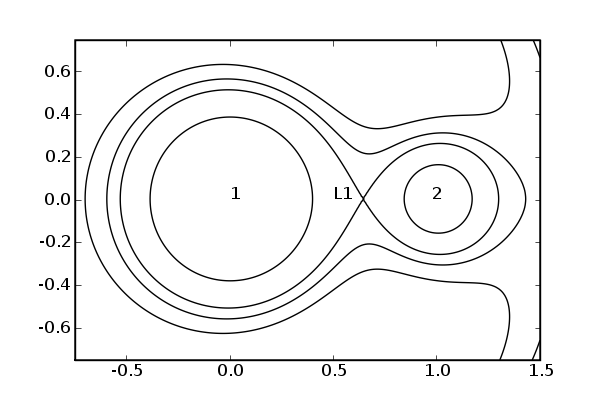
\includegraphics[width=0.85\columnwidth,bb=0 0 600 400]{images/roche.png}
 % roche.png: 600x400 pixel, 72dpi, 21.17x14.11 cm, bb=0 0 600 400
 \caption[Plot of Roche surface]{Plot of the Roche surfaces for a system with $\frac{M_{2}}{M_{1}}  = 0.25$ and $P = 4$ hours. The axes are labelled in units of binary separation. The labels ``1'' and ``2'' indicates positions of the white dwarf and red dwarf stars respectively.}
 \label{roche}
\end{figure}


\section{Formation of Cataclysmic Variables}


Cataclysmic variable stars are thought to form from a binary system in which the one star is more massive than the other. The more massive star (primary) depletes its hydrogen storage and evolves to the red giant stage. This results in an expansion of the envelope of the primary, leading to a common-envelope stage where the outer layers of the now-expanded primary contains the orbit of the secondary star. The increased aerodynamic friction on the secondary star causes angular momentum to be transferred from the secondary star to the outer layers of the expanded primary. The increase in the angular momentum causes the ejection of the outer layers of the primary into the interstellar medium. This process happens relatively quickly and ends in a pre-cataclysmic variable system which consists of a main sequence secondary orbiting the hot core of the primary star (subdwarf). The system is now detached \citep{warnerbible}.

In order for the orbit to decay further, a different mechanism of angular momentum loss is needed. The most likely possibilities are magnetic braking and gravitational radiation. It has been shown that magnetic braking is a more efficient mechanism of angular momentum loss than gravitational radiation for this stage of evolution of these stars and is therefore the mechanism driving angular momentum loss at this stage \citep{magbrake}.

Main sequence stars have solar winds consisting of particles being ejected at supersonic velocities. These particles are charged and must move along the star's magnetic field lines. Since the secondary star is rotating, the field lines are forced to rotate with it. The particles on the field lines provide a torque on the secondary star, opposing the rotation. This causes angular momentum loss and a subsequent decay of the orbit. When the orbit has decayed sufficiently, the secondary will fill its Roche-lobe and mass transfer commences. The system is now a semi-detached binary with stable mass transfer.


\section{Evolution of Cataclysmic Variables}

Cataclysmic variables undergo evolutionary changes. The main mechanisms for the evolution are mass transfer, magnetic braking and gravitational radiation. A histogram of all known cataclysmic variables shows a significantly lower number of systems with orbital periods between $\sim$2 and $\sim$3 hours than systems outside this range \citep{baraffekolb}. This is called the period-gap. For systems above the period-gap, magnetic braking is the mechanism which causes the orbital period to decrease. For the systems below the period-gap the mechanism is gravitational radiation.

The evolution of the orbital period works as follows. Mass is transferred from the secondary to the primary, carrying angular momentum with it.  The orbital separation increases and the secondary star shrinks by an infinitesimal amount and gets out of contact with its Roche-lobe. However, magnetic braking causes a decrease in orbital separation in order to conserve angular momentum. The  secondary therefore moves into contact with its Roche-lobe again. This is a continuous process and results in stable mass transfer and a decrease of the orbital period.

The mass transfer causes the convective zone of the secondary to become deeper over time. It is thought that at orbital periods of $\sim$3 hours, the convective core becomes deep enough to cause a sharp decrease in the solar wind outflow. The result is a sharp decrease in the mass transfer rate, because magnetic braking is no longer responsible for the angular momentum transfer \citep{warnerbible}. This is the so-called disrupted magnetic braking model \citep{baraffekolb}. At this stage the dominant mechanism for angular momentum transfer is gravitational radiation which becomes more efficient at lower orbital periods. At orbital periods of $\sim$2 hours, the secondary star moves into contact with its Roche-lobe and mass transfer can commence. The mass transfer rate is now lower than before the system evolved into the period-gap because gravitational radiation is less efficient at transferring angular momentum than magnetic braking.


%#########################################################
% Finish this!
% 
% 
% The angular momentum loss mechanism is still poorly understood. Recent studies show the evolution for systems below the perithe disrupted magnetic braking model 

%#########################################################


There is an observed period-minimum in the population of dwarf novae. This can be explained by evolution of the secondary to a point where it becomes semi-degenerate. Gravitational radiation causes the orbital period to decrease in the same manner as before. At an orbital period of $\sim$80 minutes, the secondary star has lost enough mass to become semi-degenerate. At this point, the orbital period starts to increase. As mass is transferred to the primary, the orbital separation increases. However, the volume of a semi-degenerate star increases slightly if mass is removed from it. This causes the secondary to fill its Roche-lobe at this increased orbital separation. The process is continuous and results in an increase in orbital period.



\section{Dwarf Nova Outbursts and Nova-likes }

\subsection{Disk Instability and Outbursts}

Long term monitoring of cataclysmic variables have shown systems that repeatedly undergo phases where the brightness of the system increases by up to 5 magnitudes. The most famous example of such a system is SS Cygni \citep{SSCyg}. These are dwarf nova outbursts and are thought to be the result of an instability in the accretion disk. 

The material transferred from the secondary builds up in the accretion disk and some of the material accretes onto the primary. The build-up of material causes the density of the disk to increase over time. This increase in density leads to an increase in the viscosity. Because viscosity is the mechanism which drives mass transfer through the disk, increased viscosity will increase the mass transfer through the disk. Material falling into a gravitational well such as this will radiate its energy away, thereby increasing the disk temperature. When the disk reaches $\approx 10000$ K the ionization of hydrogen causes the disk to become optically thick and absorb photons very efficiently. This causes a runaway reaction whereby the disk becomes fully ionized. The mass transfer rate will now commence at a high rate and dump a large amount of material onto the white dwarf. However, the rate of cooling in this `high-state' disk exceeds the rate of heating and the disk will gradually cool off. When it reaches the point where hydrogen can recombine, the disk starts cooling rapidly and returns to its quiescent state. 



\subsection{Nova-like Variables}
\label{novalikes}

A different scenario is possible for the state of the accretion disk. If the mass transfer rate is high enough, the disk can be permanently held in a high state i.e. the system is in permanent outburst. These systems are called nova-like (NL) variables. An example of such as system is V348 Puppis \citep{v348pup}. They generally have orbital periods between 3 and 4 hours. These stars have a relatively constant brightness and do not show outbursts like the dwarf novae.

The accepted classification of NLs are given in \cite{dhillon_NL} and \cite{warnerbible}. The NL systems that are not classified as magnetic systems are the UX Ursae Majoris (UX UMa) stars and the RW Tri stars. They show absorption and emission lines, respectively. See \cite{Knigge_HST_UX_UMa} for a study of the UX UMa prototype star. Some UX UMa stars enter states of low brightness. These  systems are called the VY Scl stars. Some UX UMa and VY Scl with high inclinations are observed with single-peaked emission lines and are classified as SW Sex stars. See \cite{swsex} for a discussion on the nature of SW Sex.


\section{Rapid Oscillations in Cataclysmic Variables}

The accretion process in cataclysmic variable stars is a rich source of variability in the brightness of these stars. The observation of flickering in the lightcurve of a stellar object is a tell-tale sign of accretion. Apart from the flickering, orbital modulation and eclipses observed in many examples of these stars, other stable signals can also be detected. In 1954, Merle Walker discovered the first coherent signal on a very short timescale in the object DQ Her \citep{dqher}.

There are three different stable rapid oscillations observed in dwarf novae during outburst, as well as in nova-like variables. These are the Dwarf Nova Oscillations (DNO), long period DNOs (lpDNO) and the Quasi-Periodic Oscillations (QPO)\citep{warner_ro2004}. Their stability is measured using the parameter $Q = \vert \dot{P}^{-1} \vert$.  $\dot{P}$ is the rate at which the period ($P$) changes.  The 71s period of DQ Her has a $ Q >  10^{12} $ \citep{warnerbible} and is associated with the spin period of the white dwarf. 

DNOs are rapid oscillations with periods generally of the order of tens of seconds. They are observed during outburst in dwarf novae as well as in nova-like variables and are sometimes stable to milliseconds over several hours, or can change their period by a few seconds in a few hours but generally have $ 10^{4} \lesssim Q \lesssim 10^{6} $ in the optical (or less for X-ray) observations \citep{warner_ro2004}. They generally have an amplitude of a few to a few tens of millimagnitudes. The current accepted, albeit untested, model for DNOs involves mass accretion onto a slipping equatorial belt on the white dwarf primary. The model is very similar to that of the Intermediate Polar (IP) model which involves a magnetically truncated accretion disk near the primary. The material moving through the disk gets threaded onto field lines near the white dwarf and accretes onto the magnetic poles of the primary \citep{warnerbible}. In the case of the Low-Inertia Magnetic Accretor (LIMA) \citep{DNOQPO_II} model for DNOs, the accretion onto the white dwarf is controlled by the magnetic field only very close to the white dwarf. The reasoning is that during quiescent states in dwarf novae with weaker fields, the magnetic field is too weak to force the star to rotate as a solid body. However, in the times of increased mass transfer during outburst, the material accretes onto the equator of the white dwarf thereby increasing the rotational velocity of this band on the star and causing it to slip. This causes a shear in the magnetic fields that are contained within this region, causing the field to increase in strength \citep{DNOQPO_II} and start enforcing magnetic accretion. This model requires the white dwarf to have a magnetic field of less than about $10^{5}$ Gauss. \cite{DNOQPO_II} also argues that the abrupt frequency changes seen in DNOs is caused by the snapping and reconnection of magnetic field lines along the rotating equatorial belt.

Oscillations with a similar timescale of stability as the DNOs but with a longer period by about a factor of 4 are the lpDNOs. See \cite{warner_ro2004} and \cite{WWP}. They can co-exist with the DNOs. Different models exist to explain the behaviour of lpDNOs and have been described in \cite{DNOQPO_VI}.

QPOs are oscillations with a much lower coherence ($Q \sim 10 $) than that of DNOs and lpDNOs \citep{WWP}. They are usually seen at periods of $\approx 15$ times the DNO period. Their low coherence makes it difficult to identify QPOs using Fourier techniques because their power is spread over a range of frequencies \citep{warner_ro2004}. It is thought that there may be several types of QPOs observed in CVs. In some stars double DNOs are observed where the beat period between the DNOs is approximately equal to the QPO period. The QPOs are thought to be caused by a progradely travelling wave in the inner parts of the accretion disk \citep{warner_ro2004}, thereby causing modulation of the lightcurve by obscuring or reprocessing light from the central source. The wave can be seen as a thickening of the accretion disk. QPOs without any obvious relation to the DNOs are also sometimes observed. These may have periods similar to the rotation period of the outer parts of high $\dot{M}$ (high mass-transfer rate) disks. The study of QPOs is made difficult by their low coherence and the inherent flickering of the accretion disk.  For an in-depth review of rapid oscillations in cataclysmic variables see \cite{warner_ro2004}.
 

\section{EC2117-54}
\label{ec2117}

EC2117-54 is a nova-like cataclysmic variable with V $\sim13.7$. It was found as an emission line object in the Edinburgh-Cape survey of blue objects in the southern hemisphere \citep{ecsurvey}. It has an orbital period of $\sim3.708$ hours and shows deep V-shaped eclipses. Spectroscopy reveals double-peaked emission lines and therefore puts the system in the RW Tri category. 

It is also known to regularly show DNOs and lpDNOs \citep{WWP}. Since it is relatively bright and shows DNOs and lpDNOs $\sim80$\% of the time, it is a perfect candidate with which to study these rapid oscillations in detail using high-speed spectroscopic and photometric methods.



\section{Aim of the project}
\label{aim}

An area of research that only became possible in the last decade, with the advent of 10m class telescopes, 
is the study of short period variations in the observed emission line and continuum flux of astronomical objects. The objects with the fastest known periodicities are neutron stars and the interacting binary systems they occur in. Since these are usually very faint and have most of their flux in the X-ray regime, they are not suitable for high-speed spectroscopic studies from the ground. 

Similar systems, but with more favourable properties for optical spectroscopy are the cataclysmic variables. They provide the perfect testbed for the study of accretion disk physics, since a large number of them are relatively bright and easily observable with some of the world's largest optical and infrared telescopes. Cataclysmic variables are known to produce stable variations with very short periods (2-40s) \citep{warnerbible}. These objects provides us with a unique opportunity to study their intrinsic properties, as well as accretion disks in general, using high time-resolution spectroscopy.

The first generation instruments (SALTICAM and the Robert Stobie Spectrograph (RSS)) installed on the Southern African Large Telescope (hereafter SALT)  are both designed to produce exceptional high time-resolution observations. This is one of the foreseen niche areas of SALT (and South African astronomy). This project's focus is to study rapid oscillations in an eclipsing cataclysmic variable star using the high-speed capability of the RSS together with high-quality photometric observations using the South African Astronomical Observatory (SAAO) 1.9m telescope. In particular, the behaviour of DNOs and lpDNOs are to be studied during times of eclipse. This will give an indication of the location in the system where these oscillations originate. The spectroscopic observations were made during the performance verification (PV) phase  of SALT and as such the RSS was not yet working optimally.



This project aims to identify and analyse the short period variations that are observed in high-speed photometric studies of CVs, using time-resolved spectroscopic observations of EC2117-54 as an example. This is not an entirely unexplored avenue. Studies of this kind have been done in the past using the Low Resolution Imaging Spectrograph (LRIS) on the Keck II telescope. See \cite{V2051Oph2001} and \cite{AEAqu2003} for examples on V2051 Oph and AE Aquarii respectively.

The task is made difficult due to the varying aperture size and vignetting during SALT observations and some techniques must be developed and tested to overcome these difficulties. This study combines high-speed photometric and high-speed spectroscopic observations to achieve the desired results.





\chapter{Photometry of EC2117-54}


\section{Observations}
\label{ch_photometry}

% This chapter describes the methods used to obtain the observational data as well as the methods used to clean, prepare and analyse the datasets.
% 
% For this project measurements of the object's brightness were taken simultaneously with its spectrum. Both the photometric and spectroscopic  measurements were obtained using short exposure times in order to have high time resolution.

\subsection{SAAO 1.9m Radcliff Reflector}

\label{saao1.9}

The photometric observations were made using the 1.9m reflector\footnote{Details of this telescope can be found at http://www.saao.ac.za/facilities/telescopes/19m/} at the South African Astronomical Observatory (SAAO) site in Sutherland. The telescope was built between 1938 and 1948 by Grubb-Parsons. It was originally situated at the Radcliff Observatory outside Pretoria, but was moved to Sutherland in the 1970s due to bad light pollution.

The telescope is equatorially mounted, and is used in a Cassegrain configuration at the f/18 focus. It can be fitted with a variety of instruments, the most common being the University of Cape Town (UCT) CCD photometer, a grating spectrograph and a fibre-fed Echelle spectrograph.



\subsection{UCT CCD Photometer}
\label{uctccd}

The UCT CCD photometer is a Wright Instruments Peltier-cooled camera. It has a 576x420 thinned, back-illuminated EEV CCD. The instrument can be used on the 1.9m, 1.0m and 0.75m telescopes at Sutherland. The instrument is controlled by a 486 computer running MS-DOS \citep{UCTCCD}.

It can be used in various configurations. The gain can be set depending on the brightness of the target objects. The gain is the ratio of photo-electrons to Analog-to-Digital units (ADU). The gain can be set to either 1 or 4 with gain 1 corresponding to 10 photo-electrons/ADU and gain 4 corresponding to 2.5 photo-electrons/ADU. This option is available to optimise signal-to-noise ratios for bright and faint stars. With the gain set to 1, a higher number of photo-electrons can be read before the analog-to-digital converter saturates. This setting is used for bright stars. On a gain setting of 4, a higher number of ADUs are read per photo-electron thereby decreasing the noise added by the readout process.  The gain was set to 4 for all the observations made for this project.

The CCD can be prebinned before the values are read out, in order to reduce readout noise and increase the signal-to-noise ratio. The instrument allows prebinning values from 1x1 to 6x6, however, using too much binning may result in stellar images that are undersampled for precise  Point Spread Function (PSF) fitting. A general rule of thumb is to  select the prebinning such that the star occupies $\sim$2.2 pixels on the output image. The image scale is 0.139 arcsec/pixel on the 1.9m telescope and generally prebinning values of 3x3 or greater are used, depending on seeing conditions.

The CCD is also equipped to perform observations in frame transfer mode. In this mode, half the CCD is masked by a frame transfer mask. The unmasked half is then exposed, after which the counts are transferred to the masked half of the CCD, where they can be read out while the unmasked area is exposed again. This minimises the downtime between exposures. The field-of-view on the 1.9m telescope in this mode is $34''$x$50''$ \citep{woudt2001HSP}. This high-speed mode was used for the observations made for this project.




\subsection{Photometric Observations in 2006}
\label{sub_observations}
Photometric observations of EC2117-54 were made on four consecutive nights from 16 to 19 August 2006. The runs on 18 and 19 August were hampered by intermittent cloud.  The observations were made using a Johnson V filter in order to provide a way of correlating the photometric and spectroscopic observations. An integration time of 6 seconds was selected. This is the highest time resolution that is reliable on this instrument and is well within the Nyquist frequency for the most rapid oscillations that were to be studied. The use of shorter integration times than $\sim6$s causes the computer controlling the camera to crash intermittently, due to the limited speed at which the frames can be transferred across the network.  The shortest timescale of the variations under study is approximately 20 seconds. According to the Nyquist sampling theorem, a signal with frequency $f_{0}$ must be sampled at a frequency of at least $2f_{0}$ to be fully resolved.  The telescope was pointed in such a way that ensured that the image contained at least one relatively bright non-variable star that could be used to calculate differential corrections (Figure \ref{exposure}). Table \ref{obslog} lists the full observation log.


%#############################################################################################################################
\begin{figure}
\centering
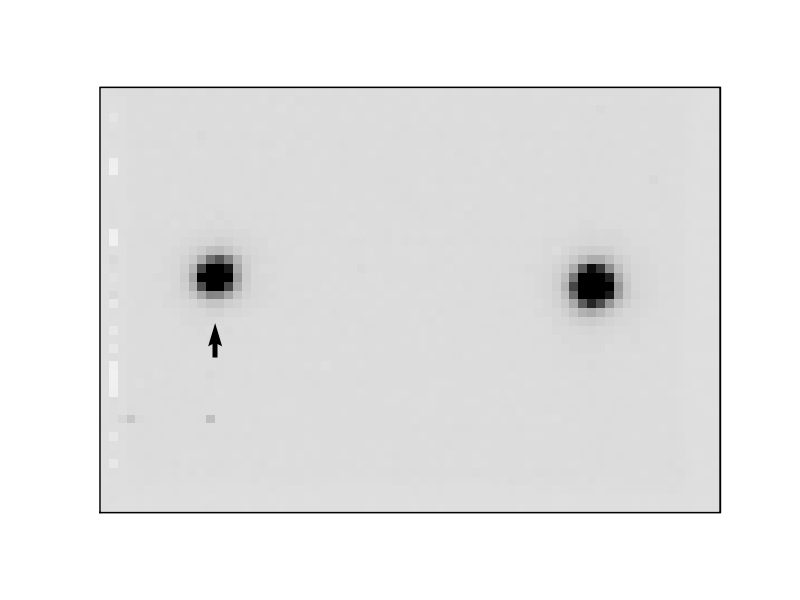
\includegraphics[bb=0 0 600 400,width=0.85\columnwidth]{images/ec2117_phot_exp.png}
% ec2117fits.png: 600x400 pixel, 72dpi, 21.17x14.11 cm, bb=0 0 600 400
\caption[Example of photometric exposure]{Example of photometric exposure of EC2117-54 and comparison star. The arrow marks EC2117-54. The field of view is $34''$x$50''$.}
\label{exposure} 
\end{figure}

\begin{table}
\caption[Photometric Observations Log]{Photometric Observations Log}
\begin{small}
\centering
% use packages: array
\begin{tabular}{lcccccc}
\hline\hline\\ Run No & Date            & HJD of first obs & Length & $t_{in}$ & Tel & Filter \\ 
        &(start of night) &     (+2453900)   &    (h)   & (s) &       & \\\\ \hline  \\
 S7651  & 16 Aug 2006     &    64.28141      &  5.35    & 6  & 74-in & V \\ 
 S7655* & 17 Aug 2006     &    65.32565      &  6.26    & 6  & 74-in & V \\  
 S7659  & 18 Aug 2006     &    66.31921      &  4.36    & 6  & 74-in & V \\ 
 S7661  & 19 Aug 2006     &    67.40985      &  0.74    & 6  & 74-in & V \\\\ \hline \\\\

\end{tabular}
Notes: $t_{in}$ = integration time, V = Johnson V filter, HJD = Heliocentric Julian Date, * = Simultaneous observations with SALT time-resolved spectroscopy.



\end{small}

\label{obslog}
\end{table}

%#############################################################################################################################
%#############################################################################################################################



%#############################################################################################################################



\subsection{Archival Observations}
\label{obs_archive}

In addition to the August 2006 observations, all lightcurves containing eclipses were retrieved from the archive\footnote{All observations of CVs obtained by UCT on SAAO telescopes are stored in an electronic archive.} in order to study the behaviour of rapid oscillations. This is further explained in Sect. \ref{ro_phot_lc}. Table \ref{archive_obslog} displays the archival runs used in the analysis. The observations were all made using the SAAO 40-inch telescope and the UCT CCD photometer. Refer to \cite{WWP} for further details of the observations.



\begin{table}
\caption[Archival Photometric Observations Log]{Archival Photometric Observations Log}
\begin{small}
\centering
% use packages: array
\begin{tabular}{lcccccc}
\hline\hline\\ Run No & Date            & HJD of first obs & Length & $t_{in}$ & Tel & Filter \\ 
        &(start of night) &        &    (h)   & (s) &       & \\\\ \hline  \\

S6544  &   07 Sept 2002   &  2452525.28604  &  6.11  &  6.0 & 40-in & WL \\
S6548  &   01 Oct 2002    &  2452549.30417  &  5.27  &  5.0 & 40-in & WL \\
S6549  &   03 Oct 2002    &  2452551.27063  &  2.34  &  6.0 & 40-in & WL \\
S6551  &   04 Oct 2002    &  2452552.27894  &  3.72  &  5.0 & 40-in & WL \\
S6555  &   06 Oct 2002    &  2452554.23099  &  1.39  &  6.0 & 40-in & WL \\
S6564  &   08 Oct 2002    &  2452556.22808  &  1.95  &  6.0 & 40-in & WL \\
S6570  &   09 Oct 2002    &  2452557.28798  &  2.53  &  5.0 & 40-in & WL \\
S6660  &   30 Nov 2002   &  2452609.26322  &  1.03  &  6.0 & 40-in & WL \\

\\ \hline \\\\

\end{tabular}
Notes: $t_{in}$ = integration time, WL = White Light, HJD = Heliocentric Julian Date.
\end{small}

\label{archive_obslog}
\end{table}







\section{Reductions}

\subsection{Photometric Measurements}

\label{phot_reductions}

The images obtained from the UCT CCD photometer are stored on a computer separate from the guide computer and the instrument's computer. They are stored in the widely used FITS (Flexible Image Transportation System) format. Before the stellar brightnesses can be measured, the images must be corrected for systematic errors. These include the non-uniform quantum efficiency of the individual pixels, dust on the CCD and filters, cosmic ray hits, dark current and bias.

The exposures are cleaned, calibrated and reduced using software based on \texttt{duphot} written by Darragh O'Donoghue. These are available on the computers at Sutherland and are used to reduce exposures ``on-the-fly'' at the telescope. The flatfields are created using the program \texttt{cleen}. The stellar brightnesses are extracted using the program \texttt{reduce}. The differential corrections are applied using the program \texttt{diffphot}.

The images have been corrected by dividing them with a master flatfield image. A master flatfield image is constructed by taking images of the twilight sky before any stars become visible. The twilight sky is essentially of uniform brightness over the field of view ($\approx 34''\times50''$) of the telescope. The telescope is set to slew mode during these exposures so as to ensure that bright stars leave a trail on the image. A large number of these images are used by calculating the median for every pixel over all the flatfield exposures, thereby ensuring that any cosmic ray hits and stellar trails will be discarded.

CCD chips are given an initial amount of electrons in the pixels to avoid having a negative value when the pixels are read out. This is called the bias. This is corrected by measuring the bias value on the overscan strip that is stored when the image is read out by the instrument, and subtracting it from the entire image.


After the images have been cleaned and calibrated, the stellar brightnesses must be measured. This is generally done in one of two ways. The most common way is to use the aperture-magnitude method. This method uses an annulus centred on a star. The radius of the annulus is chosen such that the inner circle contains the entire stellar image, and the annulus contains only the sky background. The counts inside the background annulus are added up and the average count per pixel is then calculated and subtracted from every pixel inside the inner circle. The pixel values in this circle are then added to give a total intensity. This gives a measure of the brightness of the star.

The second method used is that of Point Spread Function (PSF) fitting. A PSF is a mathematical function which represents the distribution of light across a stellar image. The PSF model is fitted to the brightest stars on an image and then scaled for every individual star. This ensures that the shape of the PSF is modelled on a high signal-to-noise ratio image. The scaled PSFs are then integrated to produce measures of stellar brightnesses.

The differentially-corrected lightcurves are shown in Figure \ref{lightcurves}. The lightcurves have been converted to intensity and normalised by their mean values. They are displayed in order from top to bottom and are vertically displaced by arbitrary amounts for display purposes. The eclipses can be seen clearly in the lightcurves.

The stellar brightness was not calibrated using a standard star because only relative brightness variations were studied, and linking to the photometric system was not needed. The SALT spectra were calibrated using a smoothed, uncalibrated lightcurve. This resulted in photometry and spectroscopy that is internally consistent but not in a particular photometric system.


%#############################################################################################################################

\begin{figure}
\begin{center}
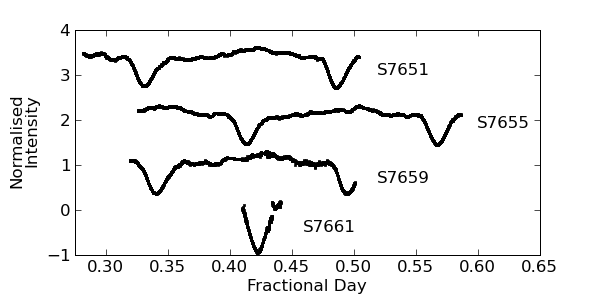
\includegraphics[bb=0 0 600 300,width=\columnwidth]{images/lightcurves.png}
 % lightcurves.png: 600x400 pixel, 72dpi, 21.17x14.11 cm, bb=0 0 600 400
\caption[Lightcurves of EC2117-54 for 16-19 August 2006.]{Lightcurves of EC2117-54 for 16-19 August 2006. They are in chronological order from top to bottom. They have been vertically displaced by arbitrary amounts for display purposes.}
\label{lightcurves}
\end{center}
\end{figure}

%#############################################################################################################################

\subsection{Ephemeris}

\label{ephemeris_section}

The August 2006 observations do not span a large enough period to precisely determine the orbital period from eclipse timing. Observations made some years earlier \citep{WWP} were retrieved from the archive and used to calculate the eclipse ephemeris. EC2117-54 shows partial eclipses, therefore only the accretion disk is being eclipsed. Because the accretion disk is subject to non-uniform variations of various causes, the eclipse profile is not the same for every eclipse. Measurement of the times of eclipse minima is therefore difficult because an identical function cannot be fitted to all eclipse profiles.

The eclipse minimum was located by finding the lowest point of a spline fitted to the eclipse. A spline fitting every 20 data points was used to find a smoothed version of the eclipse. This calculation was performed using a program written in the \texttt{Python} language.



% took the following approach,Fit a cubic spline through every $N$ datapoints in the eclipse.
% Evaluate the spline.
% Find the minimum value of the spline using a minimum slope algorithm.

%#############################################################################################################################

\begin{figure}
\begin{center}
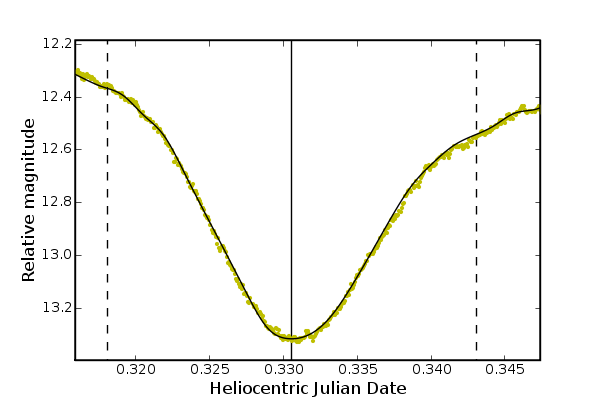
\includegraphics[width=0.85\columnwidth,bb=0 0 600 400]{images/eclipseminimum.png}
 % eclipseminimum.png: 600x400 pixel, 72dpi, 21.17x14.11 cm, bb=0 0 600 400
\caption[Measurement of eclipse minimum]{The plot shows the first eclipse in run S7651 (yellow/grey dots), the superimposed smoothing spline (solid black curve) and the date of the measured minimum (solid black vertical line). The broken lines on either side of the solid black vertical line are the limits between which the software finds the minimum. The magnitudes are instrumental. The number 2453964 has been subtracted from the Heliocentric Julian date.  }
\label{eclipseminimum}
\end{center}
\end{figure}

%#############################################################################################################################

Figure \ref{eclipseminimum} shows an example of the smoothing spline fitted to an eclipse and the corresponding minimum value found using this method. This is then repeated for all of the eclipses. Careful records must be kept of the number of eclipses that occurred after the first eclipse, to ensure that no cycle slips occur. Cycle slips show up as big residuals in the least-squares calculation. 

A first order function is then fitted to the eclipse times using least-squares to derive a precise value of the period. A parametric least-squares adjustment was used to estimate the period and its standard error. The method is outlined below.

The function to be fitted is written in the following form: $$  v = Ax - l $$ where $x$ contains unknowns, $v$ contains the residuals, $l$ contains the measured values and $A$ contains the coefficients of the unknowns. It can then be shown that the best-fit values of $x$ are given by $$ x = (A^{T}A)^{-1}A^{T}l $$ where $A^{T}$ denotes the matrix transpose of $A$. 

It can also be shown that the error estimates can be calculate from the following relation, $$ \Sigma_{xx} = \sigma^{2}_{0} \Sigma $$ where $$ \Sigma = (A^{T}A)^{-1} $$ and $$ \sigma^{2}_{0} = \frac{v^{T}v}{n-u} $$ where $n-u$ is the degrees of freedom of the solution. The matrix $ \Sigma_{xx} $ is known as the \textit{variance-covariance} matrix. The diagonals in this matrix contain the variances of the unknowns and the off-diagonal terms contain the covariances.

%#############################################################################################################################

\begin{figure}
\begin{center}
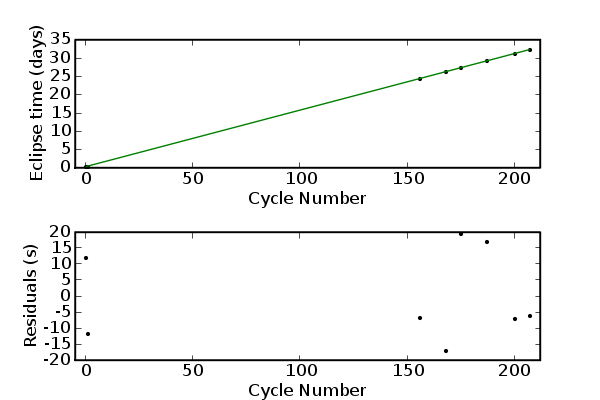
\includegraphics[width=0.80\columnwidth,bb=0 0 600 400]{images/ephemplot.png}
% ephemeris.png: 600x400 pixel, 72dpi, 21.17x14.11 cm, bb=0 0 600 400
\caption[Plot of Eclipse times versus cycle number of archival data]{The top plot shows eclipse times (in days) versus cycle number and the best-fit ephemeris, see Equation \ref{archive_ephem}. The bottom plot shows the residuals after the best-fit line has been subtracted.  The plots are based on the 2003 archival data.}
\label{ephemeris}
\end{center}
\end{figure}


\begin{figure}
\begin{center}
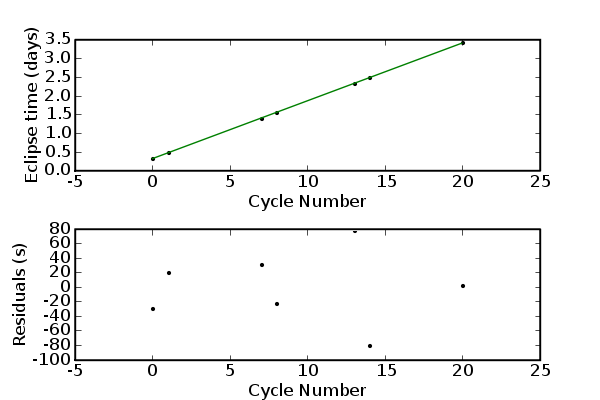
\includegraphics[width=0.80\columnwidth,bb=0 0 600 400]{images/ephem_plot_aug_data.png}
% ephemeris.png: 600x400 pixel, 72dpi, 21.17x14.11 cm, bb=0 0 600 400
\caption[Plot of Eclipse times versus cycle number of August 2006 data]{The top plot shows eclipse times (in days) versus cycle number and the best-fit ephemeris, see Equation \ref{aug_ephem}. The bottom plot shows the residuals after the best-fit line has been subtracted. The unit on the ordinate is seconds. The plots are based on the August 2006 data.}
\label{ephemeris_aug}
\end{center}
\end{figure}

%#############################################################################################################################

% The result from this method gives the period as $$ P = 13351.06 \hspace{4pt}s \pm 0.07 \hspace{4pt}s $$ where all the units are in seconds. See Figure \ref{ephemeris}.  

The ephemeris calculated from the archival data is given by
\begin{equation}
	\textrm{HJD}\:\: 2452525.374416 \pm 2 \times 10^{-4} + 0.154525E \pm  1\times 10^{-6}.
\label{archive_ephem}
\end{equation}

The bottom panel of Fig. \ref{ephemeris} shows the residuals of best fit ephemeris based on the 2003 archival data.  After this has been done for all the available eclipses, the resulting eclipse times and cycle numbers are plotted (see top panel of Fig. \ref{ephemeris}). Over the timescale of these measurements ($\approx$ 30 days), the eclipse times versus cycle number is a straight line.

The zero-point for the 2006 eclipse ephemeris was recalculated on the first eclipse of run S7651 and the new ephemeris is

\begin{equation}
	\textrm{HJD}\:\: 2453964.330709 \pm 4 \times 10^{-4} + 0.154525E \pm  1\times 10^{-6}.
\label{aug_ephem}
\end{equation}

The ephemerides are given in Heliocentric Julian Date. The orbital period and all errors are given in days. The errors are $1\sigma$ errors found from a least-squares fit. The orbital period and its error are those calculated from the 2003 archival data. Figure \ref{ephemeris_aug} displays the residuals of the ephemeris calculation based on the August 2006 observations. The residuals from the August 2006 fit contain 2 points with residuals that are much larger than the other eclipses. The ephemeris is measured using the minimum brightness during eclipse. The minimum brightness during eclipse in cataclysmic variables may occur at imprecise times due to flickering, noisy observations and other factors causing a non-uniform brightness distribution in the accretion disk.

The calculations were made using a program written using the \texttt{Python} programming language and the extension libraries, \texttt{Scipy} and \texttt{Matplotlib}. The spline minimum was calculated using the \texttt{Scipy} function, \texttt{fminbound}.

\section{Methods}
\subsection{Flattening of Lightcurves}

\label{flat_section}

The photometric observations were made in order to identify certain periodic phenomena in the brightness of the object. This was done using the standard method of Fourier analysis techniques. Periodograms of the lightcurves were calculated and the DNOs and lpDNOs were identified as peaks above the noise level. However, since the object undergoes an eclipse approximately every 3.708 hours, large low-frequency peaks appear in the periodograms that can suppress low amplitude peaks in the periodogram. This is illustrated in the periodogram shown in the bottom panel of Fig. \ref{unflat}. The lightcurves were flattened to remove variations in the brightness profile that are caused by the object's orbit.

All lightcurves were converted to intensity units and normalised their mean value. This allows for direct comparison of oscillation amplitudes between runs that is not dependent on the magnitude zero-point.

Different methods to remove the long period (orbital) variations from the lightcurves were investigated. The first method involved fitting a smoothing spline to the lightcurve and then subtracting it. This method removed the slow variations quite well but involved manual fitting of the spline to each lightcurve. In addition, this method gives no guarantee that periodic phenomena are not altered by the subtraction of the smoothing spline. This method was therefore deemed unsatisfactory.

Fast Fourier Transforms (FFTs) were used to remove the long period variations from the lightcurves. This requires the lightcurves to be sampled at regular intervals, which is not necessarily the case in astronomical observations. The lightcurves that contain gaps were interpolated to a regular grid using linear splines. The FFTs of the lightcurves were calculated. The positive and negative frequency terms corresponding to the long period signals were then set to zero, after which the inverse Fast Fourier Transform was calculated. This returns the lightcurve with the orbital variation and other longer period signals removed. Signals with a period longer than 30 minutes were removed because the rapid oscillations of interest have periods much shorter than this. This method resulted in flattened lightcurves with significant edge effects, caused by the discontinuity at the endpoints of the lightcurve i.e. the values of the lightcurve did not tend to zero at the start and end. For this reason, this method was also deemed unsatisfactory.

The method that was ultimately decided on involved the use of digital infinite impulse response (IIR) filters. This is the optimal way of removing unwanted frequencies from a signal. It has the advantage that the filter response, i.e. the attenuation as a function of frequency, is known. A ``Chebychev'' filter of Type I was used to construct a high-pass filter with a passband from 144 cycles/day, a transition-band between 100 and 144 cycles/day and a stopband below 100 cycles/day. The minimum attenuation in the stop band is 15 dB and the maximum attenuation in the pass band is 0.1 dB. A \texttt{Python} program using the \texttt{Scipy} package was used to implement this filter.

Figure \ref{unflat} shows a raw lightcurve and its periodogram. The noise level is at $\sim 0.1\%$ and no significant peaks at higher frequencies can be discerned. Figure \ref{flat} shows the same lightcurve from before, after it has been flattened with the IIR filter and its periodogram. The noise level is much lower than before ($< 0.001$) and the shorter period peaks can now clearly be identified.



%######################################################################################################################
\begin{figure}
\begin{center}
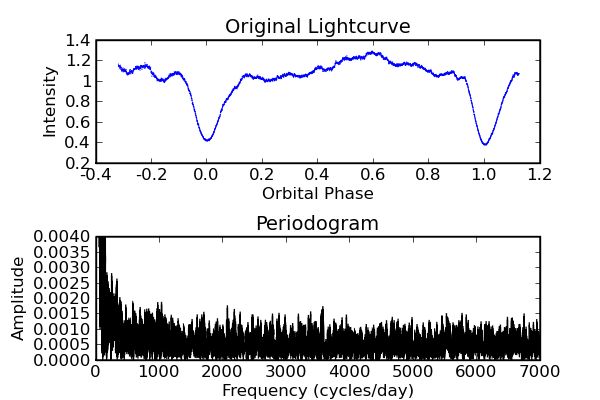
\includegraphics[width=0.80\columnwidth,bb=0 0 600 400]{images/unflattened.png}
 % unflattened.png: 600x400 pixel, 72dpi, 21.17x14.11 cm, bb=0 0 600 400
\caption[Original lightcurve and periodogram]{The original lightcurve of run S7651 and its periodogram. The periodogram is totally dominated by low-frequency noise and no details can be discerned.}
\label{unflat}
\end{center}
\end{figure}

%######################################################################################################################
%######################################################################################################################

\begin{figure}
\begin{center}
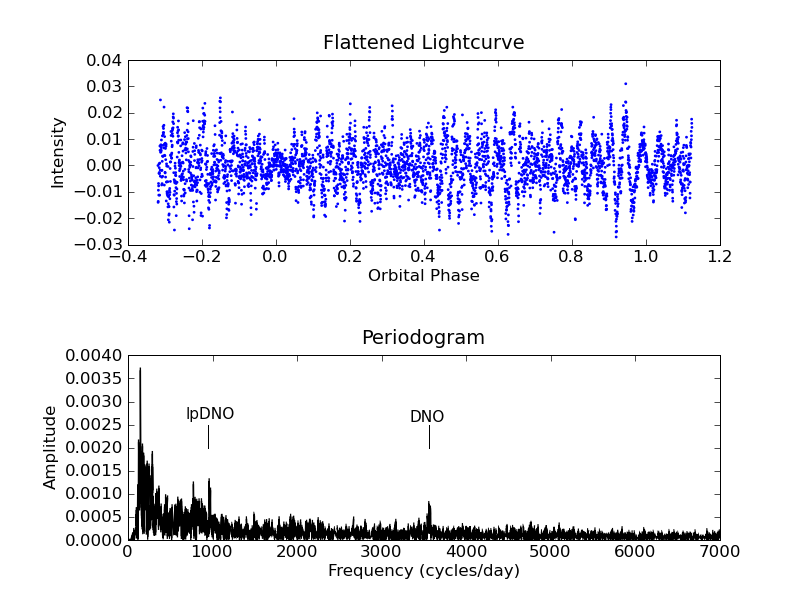
\includegraphics[width=0.80\columnwidth,bb=0 0 600 400]{images/flattened.png}
% flattened.png: 600x400 pixel, 72dpi, 21.17x14.11 cm, bb=0 0 600 400

\caption[Flattened lightcurve and periodogram]{The ``flattened'' lightcurve of run S7651 and its associated periodogram. Details in the periodogram can now be identified. Note the DNO peak at $\approx 3600$ cycles/day and lpDNO peak at $\approx1000$ cycles/day. The lightcurve was filtered using the IIR-filtering method described in Sect. \ref{flat_section}. }
\label{flat}
\end{center}
\end{figure}

%######################################################################################################################

% The lightcurves were ``flattened'' by calculating a smoothing spline fitting every $N$ points. The spline was then evaluated at the same times the observations were made at. The resulting points obtained from the spline were subtracted from the lightcurve to produce the ``flattened'' lightcurve. Cubic splines were again used for this operation. They were typically fitted to every 40 - 80 points (corresponding to 240 - 480 seconds). See Figure \ref{splineandflat} for an example.


\subsection{$O-C$ Diagrams}

\label{ominc_section}

In order to study the evolution of DNOs and lpDNOs, it is necessary to track the changes in their amplitude and phase as a function of time. This was done for this project using the following technique.

The lightcurves were flattened using the digital filtering technique described in Section \ref{flat_section}. The periodogram of the flattened lightcurve was then calculated and the frequencies at which the DNO and lpDNO peaks occurred were noted. An \textit{Observed - Calculated} ($O-C$) diagram was then plotted of the DNO or lpDNO at the frequencies found in the periodogram.

%#############################################################################################################################

\begin{figure}
 \centering
 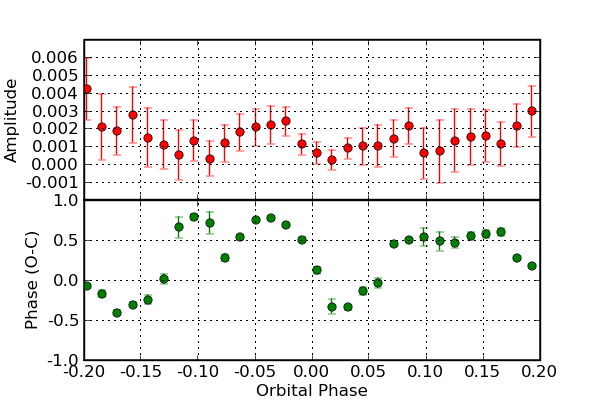
\includegraphics[width = 0.8\columnwidth, bb=0 0 600 400]{images/august_phot/S7651/S7651_24.30.png}
 % vel_ew.png: 1179666x1179666 pixel, 0dpi, infxinf cm, bb=0 0 600 400
 \caption[$O-C$ diagram around the first eclipse of run S7651.]{$O-C$ diagram around the first eclipse of run S7651. The phase was calculated relative to a signal with constant period of 24.30s (3555.56 cycles/day) using 15 cycles and 50\% overlap.  }
 \label{OC_example}
\end{figure}

%#############################################################################################################################

The $O-C$  diagrams are calculated by fitting a \textit{sine} function with the DNO period to overlapping segments of the lightcurve. The amplitude and the phase of the \textit{sine} function are allowed to vary. Their time-evolution can therefore be studied. The amount of overlap was chosen to be $50\%$, in order to minimise fitting error and to sample the lightcurve at closer intervals. Each segment typically contains $5$ to $40$ cycles of the variation under inspection. Knowing the sampling rate of the data, the frequency to be studied and the number of cycles to use in the process, it is trivial to calculate the number of data points to use for a segment. The fitting function used for the $O-C$ diagrams is $$y(t) = Acos(2\pi Ft) + Bsin(2\pi Ft)$$ where $F$ is frequency, $$Amplitude =\sqrt{A^{2} + B^{2}} $$ and $$ \phi = arctan(\frac{-B}{A}) $$
The amplitude and phase were then plotted as a function of time. Figure \ref{OC_example} shows the $O-C$ diagram for a DNO in run S7651. The fitting was done using the method described in section \ref{ephemeris_section}.

%#############################################################################################################################

\begin{figure}
 \centering
 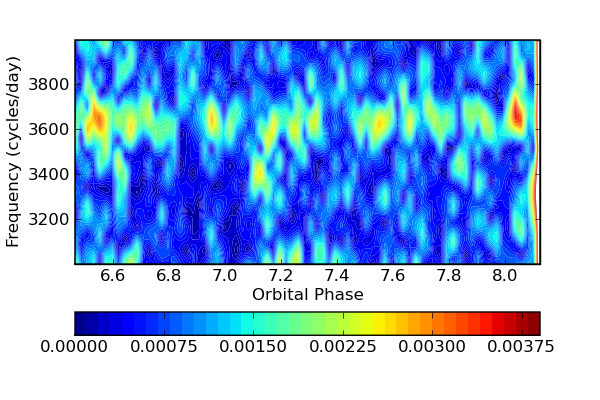
\includegraphics[width = 0.8\columnwidth, bb=0 0 600 400]{images/august_phot/S7655/S7655_DNO_trailed_FT.png}
 % vel_ew.png: 1179666x1179666 pixel, 0dpi, infxinf cm, bb=0 0 600 400
 \caption[Spectrogram for run S7655.]{A spectrogram for run S7655 around the $\sim3600$ cycle/day frequency. The color-bar shows the amplitude values in normalised intensity.  }


 \label{trailed_ft_example}
\end{figure}

%#############################################################################################################################


Examination of $O-C$ diagrams may reveal changes in the frequency and amplitude of an oscillation. A change of frequency will show up as a slope change on the $phase$ versus $time$ plot.

\subsection{Spectrograms}
\label{spectrogram_section}
A different way of looking at frequency and amplitude changes in a signal is to use a spectrogram. The spectrograms used in this analysis were computed by calculating periodograms of segments of a lightcurve with consecutive segments overlapping by 50\%. The periodograms were then plotted in an image with the vertical axis displaying frequency, the horizontal axis displaying time and the image value displaying amplitude. The time for each periodgram (i.e. column) was calculated by taking the average value of the times in the segment. See Fig. \ref{trailed_ft_example} for an example. Periodograms were calculated using the algorithm in \cite{kurtz_ft}.








%#############################################################################################################################

\begin{figure}[t]
\begin{narrow}{-0.75	in}{0in}
\begin{tabular}{lr}
 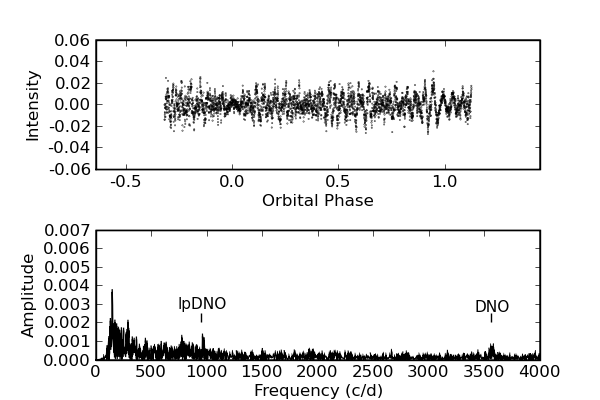
\includegraphics[width = 0.6\columnwidth, bb=0 0 600 400]{images/august_phot/S7651/S7651.png} & 
 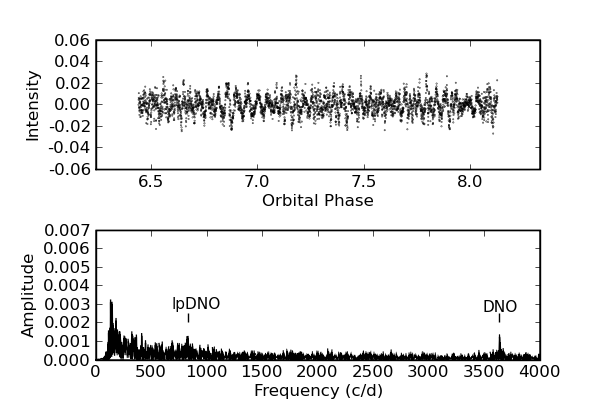
\includegraphics[width = 0.6\columnwidth, bb=0 0 600 400]{images/august_phot/S7655/S7655.png}  \\
 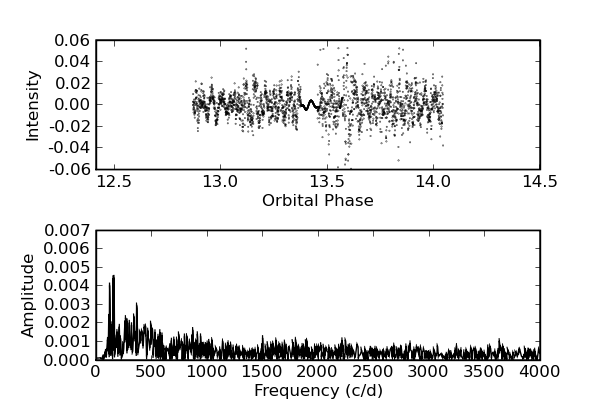
\includegraphics[width = 0.6\columnwidth, bb=0 0 600 400]{images/august_phot/S7659/S7659.png} &
 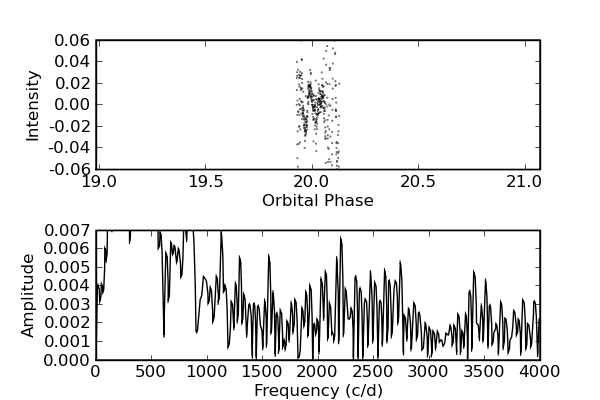
\includegraphics[width = 0.6\columnwidth, bb=0 0 600 400]{images/august_phot/S7661/S7661.png}
\end{tabular}
\end{narrow}
\caption[Flattened lightcurves and periodograms of EC2117-54.]{Flattened lightcurves and periodograms 
of EC2117-54. Clockwise from Top-left: Run S7651, S7655, S7661, S7659.} 
\label{ec2117_zcha}

\end{figure}

%#############################################################################################################################



\section{Analysis}

\subsection{Rapid Oscillations in August 2006 photometric lightcurves}
\label{ro_phot_lc}

Lightcurves from all 4 nights were flattened using the method described in section \ref{flat_section}. Periodograms were then calculated in order to identify any DNOs and lpDNOs. No search was made for QPOs because of their highly non-stationary nature. The filtering process may also introduce false signals into the lightcurve because the filter-cutoff is very close to the expected QPO period. Some of the flattened lightcurves contain sections that resembles QPOs (see top right panel of Fig. \ref{ec2117_zcha} for an example). For the above mentioned reasons these signals were ignored.  A more complete survey for them can be made using methods that incorporate non-stationarity of signal \citep{blackman}. The algorithm in \cite{kurtz_ft} was used to calculate the periodograms shown in Fig. \ref{ec2117_zcha}. The DNO ($\sim3600$ cycles/day) and lpDNO($\sim1000$ cycles/day) spikes in the periodogram can clearly be seen in run S7651 and S7655. On the third night (Run S7659) the DNOs and lpDNOs were not visible. Run S7661 was hampered by cloud and only a very short observing run was possible. The data from this run were not used in any further analyses. The DNOs and lpDNOs identified in the photometric lightcurves are shown in Table \ref{RO_table}.

%######################################################################################################################

\begin{table}
\begin{scriptsize}
\centering
\caption[Rapid Oscillations in photometry]{Rapid Oscillations in photometry.}
% use packages: array,supertabular
\begin{tabular}{rccccc}
\hline \hline\\
Run    & DNO period & DNO freq      & lpDNO period & lpDNO freq     \\ 
       & (s)        &  (cycles/day) &  (s)         &  (cycles/day)   \\ 
\\\hline \\
S7651$^{a}$  & 24.30, 24.12 [0.01] & 3555.56, 3582.09 [0.60] &  89.94 [0.01]  &  964.64 [0.60]  \\ 
*S7655$^{a}$ & 23.77 [0.30] & 3634.84 [0.01] & 104.2 [0.01] & 829.17 [0.30] \\ 
S7659$^{a}$  & --- & --- & --- &---\\ 
S7661$^{a}$  & --- & --- & --- &---\\
\hline\\
S6544$^{b}$  & 23.13 [0.03] & 3735.41 [0.70] & 95.68 [0.01] & 909.00 [0.40] \\
S6548$^{b}$  & ---   & ---     & ---    &---	\\
S6549$^{b}$  & 22.60 [0.10] & 3823.01 [2.20] & ---    &---	\\
S6551$^{b}$  & 22.66 [0.05] & 3812.89 [1.10] & ---    &---	 \\
S6555$^{b}$  & ---   & ---     & ---    &---	 \\
S6564$^{b}$  & 22.68 [0.16] & 3809.52 [3.60] & 95.39 [0.025] & 907.76 [2.40]  \\
S6570$^{b}$  & 22.63 [0.06] & 3817.94 [1.40] & 95.96 [0.014]  & 900.38 [1.30] \\
S6660$^{b}$  & 23.16 [0.15] & 3730.57 [3.40] & ---    &---     \\\\

\hline




\end{tabular}\\
* Observed in parallel with SALT high-speed spectroscopy. $^{a}$ August 2006 observing run. $^{b}$ Retrieved from archive. Errors are given in square brackets.

\label{RO_table}
\end{scriptsize}
% \caption{}
\end{table}

%######################################################################################################################



% DNO FTs

The periodogram of the flattened lightcurve of run S7651 (top left panel of Fig. \ref{ec2117_zcha}) shows evidence for a DNOs with periods at $\sim$24.3s and $\sim$24.1s. These oscillations are not present simultaneously. Calculating separate periodograms (not shown) for the first and second halves of the run reveals peaks at periods of $\sim24.3$s and $\sim24.1$s respectively.  (Table \ref{RO_table}). A very strong peak near 3640 cycles/day (23.7s) is seen in the periodogram (top right panel of Fig. \ref{ec2117_zcha}) of the flattened lightcurve of run S7655.






%######################################################################################################################

\begin{figure}[t]
\begin{narrow}{-1in}{0in}
% want 2x1 table with 2 Figs side by side on top and 1 on the bottom
\begin{tabular}{c}
    \begin{tabular}{cc}
    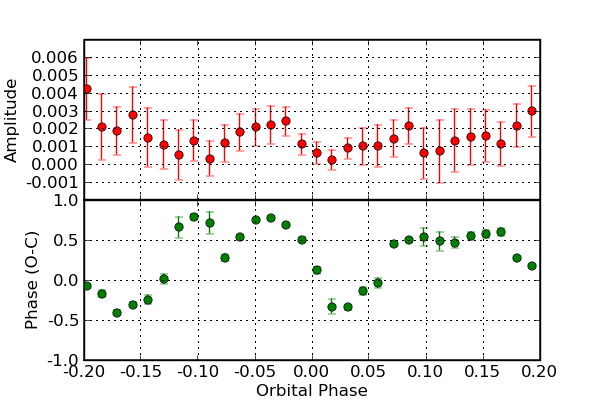
\includegraphics[width=0.65\columnwidth, bb=0 0 600 400]{images/august_phot/S7651/S7651_24.30.png} &
    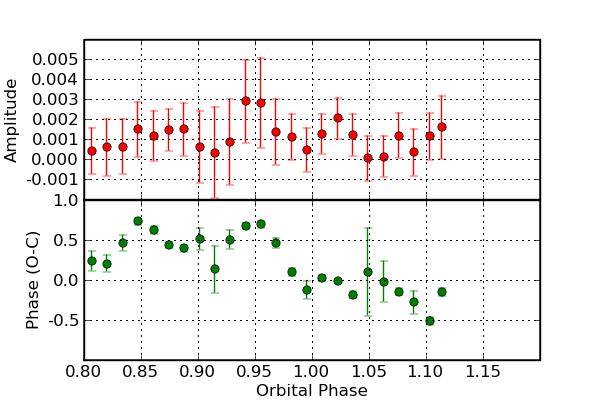
\includegraphics[width=0.65\columnwidth, bb=0 0 600 400]{images/august_phot/S7651/S7651_24.12.fixed.png}
    \end{tabular} \\
    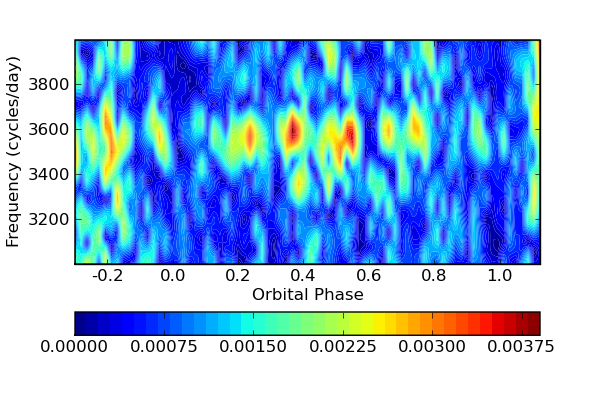
\includegraphics[width=0.65\columnwidth, bb=0 0 600 400]{images/august_phot/S7651/S7651_trailed_ft.png} 
%     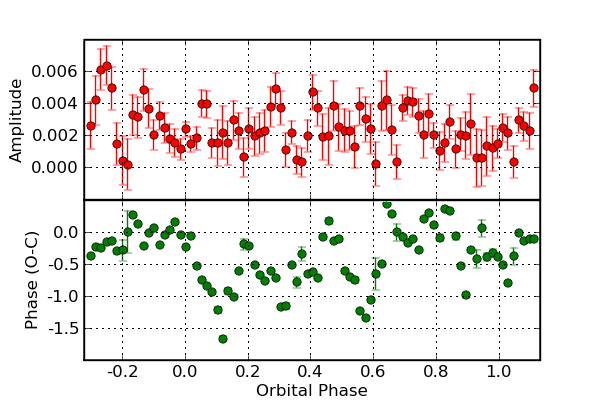
\includegraphics[width=0.42\columnwidth, bb=0 0 600 400]{images/august_phot/S7651/S7651_89.94.png}
\end{tabular}
\end{narrow}
\caption[$O-C$ Diagrams and spectrograms of DNO in run S7651]{$O-C$ Diagrams and spectrograms of DNOs in run S7651. The top left and top right panels show the $O-C$ diagrams around the first and second eclipses. They were calculated relative to signals with periods 24.3s and 24.12s respectively, using 20 cycles with 50\% overlap. The bottom panel shows the spectrogram centred on the DNO frequency for the entire run.}
\label{S7651_DNO}
\end{figure}

%######################################################################################################################




% lpDNO FTs

In the periodogram of the flattened lightcurve of run S7651 (top left panel of Fig. \ref{ec2117_zcha}, there is a very prominent peak near 960 cycles/day (89.95s). This is very close to $4\times\nu_{DNO}$ ($\nu_{DNO}= $ DNO frequency) and is therefore classified as a lpDNO. The periodogram of run S7655 showing a peak near 830 cycles/day (104.2s) can be seen in the top right panel of Fig. \ref{ec2117_zcha}. This is classified as a lpDNO and has the longest known period of all lpDNOs observed in this object. 

The DNOs and lpDNOs identified in the August 2006 runs occur at the expected periods, based on previous studies of this star \citep{WWP}. The DNOs and lpDNOs have periods of $\sim23$s and $\sim90$s respectively.



% DNO O-C
The $O-C$ diagrams of the DNO in run S7651 (top panels of Fig. \ref{S7651_DNO}) show evidence of a systematic phase change during the eclipses. The same phase variation is not seen in both eclipses of run S7651. During the first eclipse (top left panel of Fig. \ref{S7651_DNO}) the phase starts at $\sim0.7$ before eclipse, changes by $\sim1$ cycle and returns to $\sim0.5$ after eclipse. Immediately before the second eclipse the phase starts at $\sim0.5$, decreases to a value of about -0.4, and returns to $\sim-0.5$ after eclipse.

In run S7655 the DNOs exhibit similar behaviour through eclipse. The $O-C$ diagrams for the two eclipses are shown in the top panels of Fig. \ref{S7655_DNO}. The top left and top right panels show the $O-C$ diagrams for the DNO during the first and second eclipses respectively. The phase changes by $\sim$ 1 cycle during the first eclipse and does not revert to the value that was present before eclipse but instead seems to decrease. During the second eclipse in run S7655 (top right panel of Fig. \ref{S7655_DNO}) the phase changes from $\sim0.0$ to $\sim-0.9$ in mid-eclipse and returns to $\sim0.0$ after the eclipse.



% lpDNO O-C
The $O-C$ diagram (top left panel of Fig. \ref{aug_lpDNOs}) shows the lpDNO to have an irregular phase which is most likely due to the low amplitude and the associated difficulty of tracking the lpDNO. The amplitude is higher than average at orbital phases $\sim$0.3 and $\sim$1.1. The $O-C$ diagram of run S7655 (top right panel of Fig. \ref{aug_lpDNOs}) shows a constant phase throughout the run (including throught the first eclipse) that is interrupted immediately before the second eclipse. The amplitude panel as well as the spectrogram display a seemingly periodic strengthening of the signal every $\sim$0.2 to $\sim$0.3 orbital phases. These increases in amplitude seem to occur at the same orbital positions as in run S7651. The reason for this is unknown and may be purely coincidental. Neither of the runs contain an lpDNO that remained stable for long enough to be tracked through an eclipse.




% O-C diagrams





% landscpe plots for S7655
%#############################################################################################################################

% \begin{landscape}
\begin{figure}
\begin{narrow}{-1in}{0in}
\begin{tabular}{c}
    \begin{tabular}{cc}
        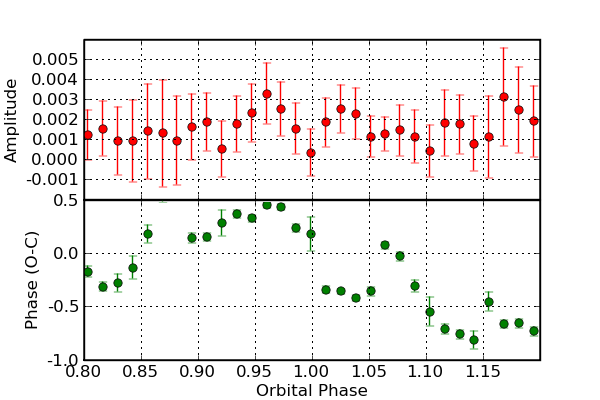
\includegraphics[width=0.65\columnwidth, bb=0 0 600 400]{images/august_phot/S7655/S7655_23.76_fixed_eclipse1.png} &
 	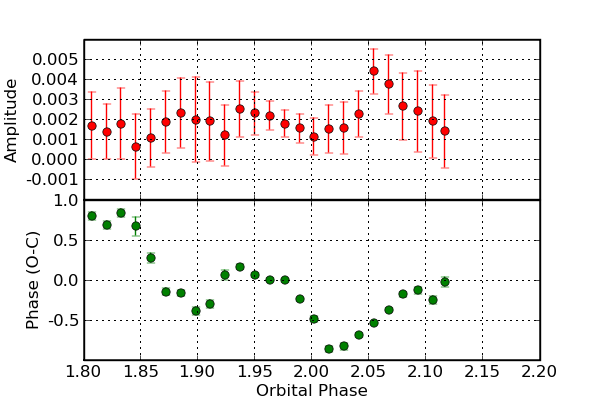
\includegraphics[width=0.65\columnwidth, bb=0 0 600 400]{images/august_phot/S7655/S7655_23.76_fixed_eclipse2.png}
    \end{tabular}  \\
 
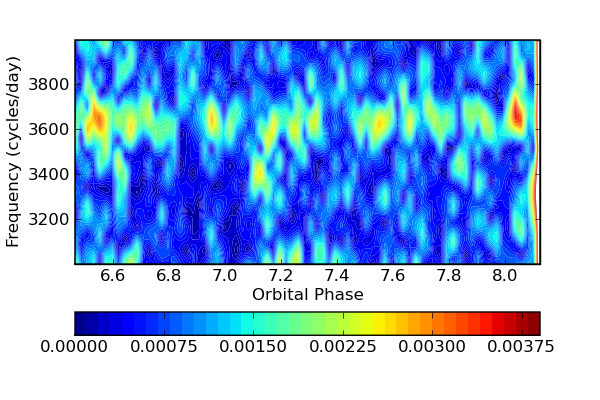
\includegraphics[width=0.65\columnwidth,bb=0 0 600 400]{images/august_phot/S7655/S7655_DNO_trailed_FT.png} 

\end{tabular}
\end{narrow}
% \end{displaymath}
\caption[$O-C$ Diagrams and Spectrograms for DNOs in run S7655]{$O-C$ Diagrams and Spectrograms for DNOs run S7655. The top left and -right panels show the $O-C$ diagrams the 23.76 s DNO during the first and second eclipse respectively. The bottom panel shows the spectrogram for the entire run centred on the DNO frequency for the entire run. The $O-C$ diagrams were calculated using 15 cycles with 50\% overlap. }
\label{S7655_DNO}
\end{figure}
% \end{landscape}

%#############################################################################################################################

\begin{figure}[t]
\begin{narrow}{-1in}{0in}
\begin{tabular}{cc}
 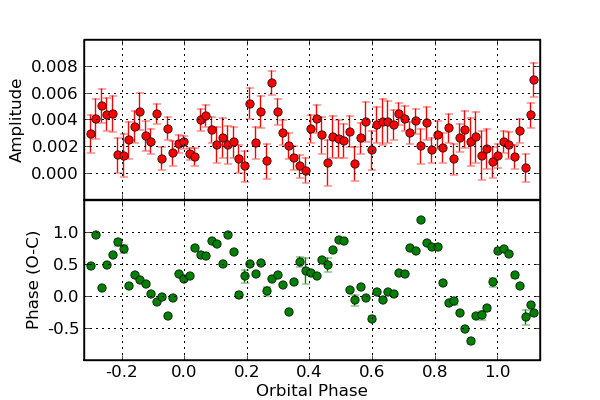
\includegraphics[width = 0.65\columnwidth, bb=0 0 600 400]{images/august_phot/S7651/S7651_89.95.png} & 
 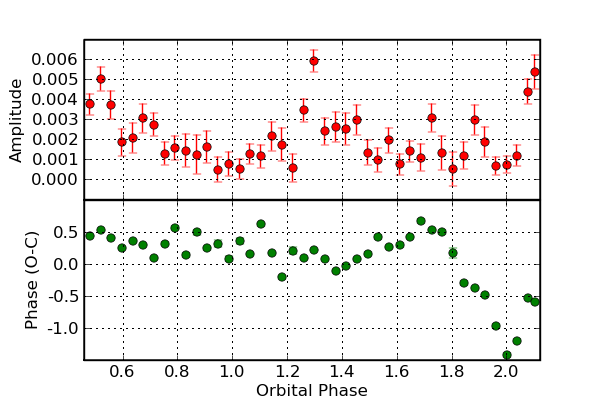
\includegraphics[width = 0.65\columnwidth, bb=0 0 600 400]{images/august_phot/S7655/S7655_104.2.png}  \\
 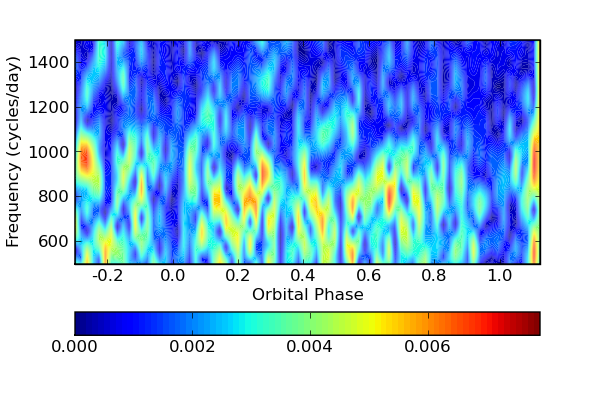
\includegraphics[width = 0.65\columnwidth, bb=0 0 600 400]{images/august_phot/S7651/S7651_trailed_FT_lpDNO.png} &
 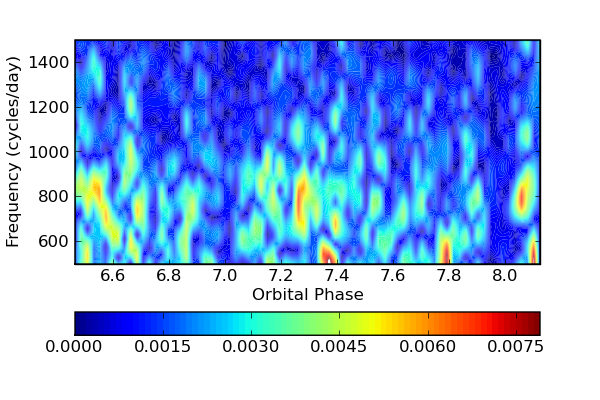
\includegraphics[width = 0.65\columnwidth, bb=0 0 600 400]{images/august_phot/S7655/S7655_lpDNO_trailed_FT.png}
\end{tabular}
\end{narrow}
\caption[$O-C$ diagrams and spectrograms of lpDNOs in EC2117-54]{$O-C$ diagrams and spectrograms of lpDNOs in EC2117-54. The left panels displays run S7651 and the right S7655.} 
\label{aug_lpDNOs}
\end{figure}




















% Z Cha



%#############################################################################################################################


Evidently the phase evolution of the DNO signal through eclipse is not visible at every eclipse. The fact that a systematic effect can be seen through eclipse suggests a geometrical origin and therefore the geometry of the system is not constant. The accretion disk, the accretion stream and the stream-disk impact zone are the only parts of the cataclysmic variable that can show changes on the timescale of an orbital cycle, and therefore one or both must have an integral part in this phenomenon. This is further discussed in Sect. \ref{photo_discussion}.



\subsection{Rapid Oscillations in archival photometric light-curves}
\label{ro_arc_phot_lc}

The discovery of systematic phase changes in the August 2006 lightcurves prompted a search for the same occurrence in data from the archive. Observations made during eclipse were retrieved and analysed using the same methods as the August 2006 data. Phase changes in the DNOs were identified in 4 of the 8 archival runs analysed (S6555, S6564, S6660 and S6570). The flattened lightcurves and their periodograms are shown in Fig. \ref{ec2117_archive}. Figures \ref{fig:ux_uma_OC} and \ref{fig:z_cha_OC} show average $O-C$ diagrams for every eclipse containing DNOs showing the two kinds of phase changes. Interestingly, the average $O-C$ diagram in Fig. \ref{fig:z_cha_OC} shows two phase changes. The first one, at orbital phase $\phi=0.9$, is shorter and more shallow than the second one ($\phi=1.05$) . This can also be seen in some of the $O-C$ diagrams of single runs. This is discussed in Sect. \ref{photo_discussion}.

A similar phase change was observed in the dwarf nova Z Cha during super-outburst by \cite{warner_brickhill}. A more modern lightcurve of Z Cha during outburst that contains DNOs was retrieved from the archive to look for the same phenomenon during eclipse. The lightcurve was flattened using the method outlined in Sect. \ref{flat_section}. Figure \ref{Z_Cha_OC} shows the filtered lightcurve and periodogram of run S6061 of Z Cha. Very strong DNOs can be seen in the periodogram (right panel of Fig. \ref{Z_Cha_OC}) at a frequency of $\sim$3500 cycles/day. This corresponds to a period of 25.15s. Examination of the $O-C$ diagram (left panel Fig. \ref{Z_Cha_OC}), calculated relative to a constant signal with a period of 25.15s, unfortunately does not show the phase changes, however, this is not surprising given the variable nature of the DNOs seen in EC2117-54.

%#############################################################################################################################

\begin{figure}
 \centering
 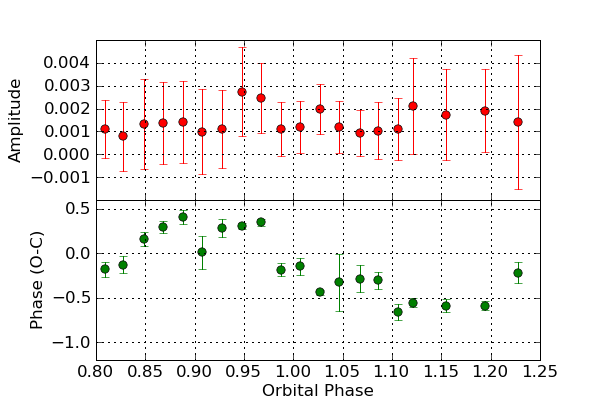
\includegraphics[width=0.7\columnwidth,bb=0 0 600 400]{images/averaged_OC/fixed_may2008/ux_uma_type/average_OC.png}
 % average_OC.png: 600x400 pixel, 100dpi, 15.24x10.16 cm, bb=0 0 600 400
 \caption[Averaged $O-C$ diagram of UX Uma-type phase change.]{Averaged $O-C$ diagram of UX Uma-type phase change. Diagram was calculated using data from run S6660, S7651 and S7655.}
 \label{fig:ux_uma_OC}
\end{figure}



\begin{figure}
 \centering
 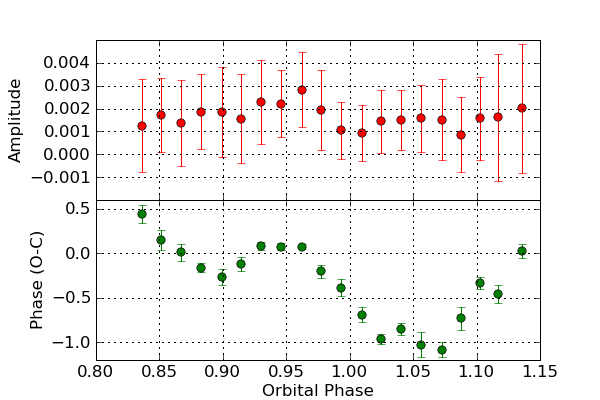
\includegraphics[width=0.7\columnwidth,bb=0 0 600 400]{images/averaged_OC/fixed_may2008/z_cha_type/average_OC.png}
 % average_OC.png: 600x400 pixel, 100dpi, 15.24x10.16 cm, bb=0 0 600 400
 \caption[Averaged $O-C$ diagram of Z Cha-type phase change.]{Averaged $O-C$ diagram of Z Cha-type phase change. Diagram was calculated using data from run S6555, S6564, S6570, S7651 and S7655.}
 \label{fig:z_cha_OC}
\end{figure}


\begin{figure}
 \centering
 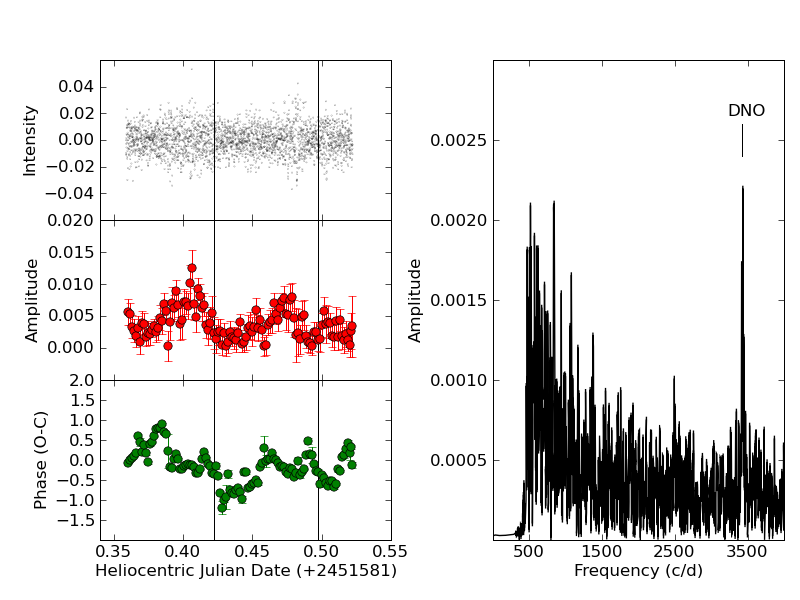
\includegraphics[width=\columnwidth,bb=0 0 800 600]{z_cha/z_cha_OC_FT.png}
 % z_cha_OC_25.13.png: 900x600 pixel, 100dpi, 22.86x15.24 cm, bb=0 0 600 400
 
 \caption[Filtered lightcurve,$O-C$ diagram and periodogram of Z Cha.]{Left: Top panel shows filtered lightcurve of run S6061 of Z Cha, middle and bottom panels contains amplitude and phase variations of the 25.15s DNO respectively. The solid vertical lines indicate times of mid-eclipse. The DNO phase change is not seen in this run. Right: Periodogram of filtered lightcurve with DNO peak marked. }
\label{Z_Cha_OC}
\end{figure}


\begin{figure}
\begin{narrow}{-0.25in}{1.5in}
\begin{tabular}{lr}
 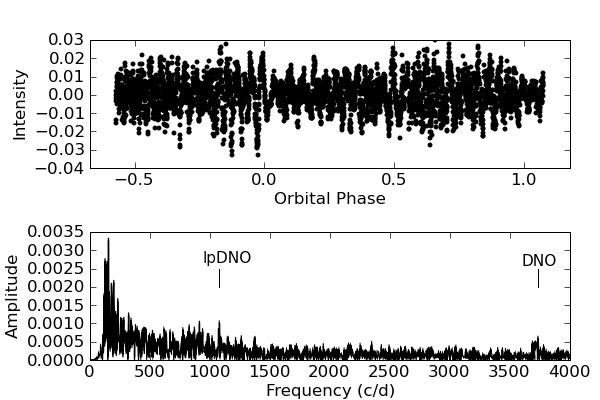
\includegraphics[width = 0.50\columnwidth, bb=0 0 600 400]{images/archive_phot/norm_int_eclipsing/S6544_c_FF.png} & 
 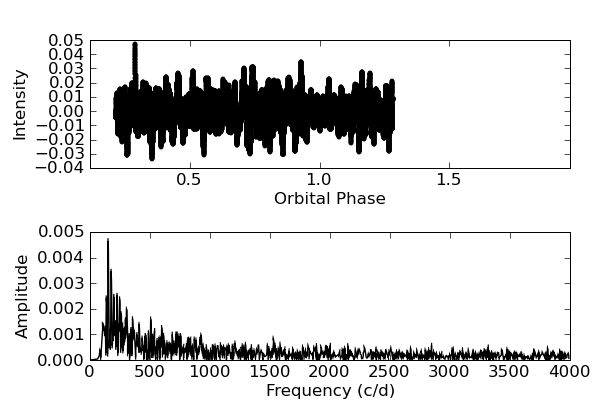
\includegraphics[width = 0.50\columnwidth, bb=0 0 600 400]{images/archive_phot/norm_int_eclipsing/S6548d_cc_FF.png}  \\
 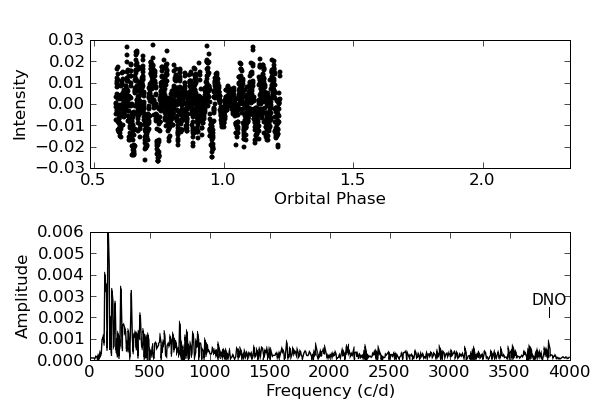
\includegraphics[width = 0.50\columnwidth, bb=0 0 600 400]{images/archive_phot/norm_int_eclipsing/S6549d_FF.png} &
 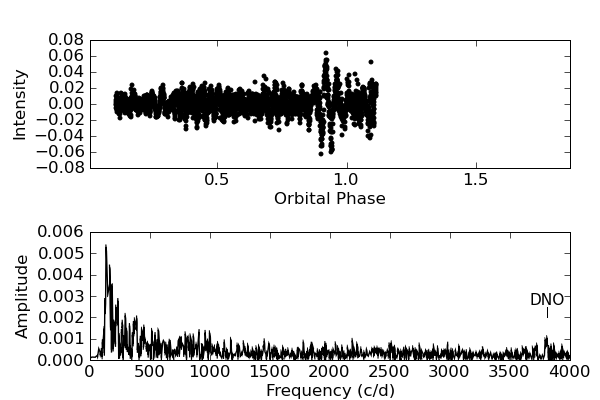
\includegraphics[width = 0.50\columnwidth, bb=0 0 600 400]{images/archive_phot/norm_int_eclipsing/S6551d_FF.png} \\
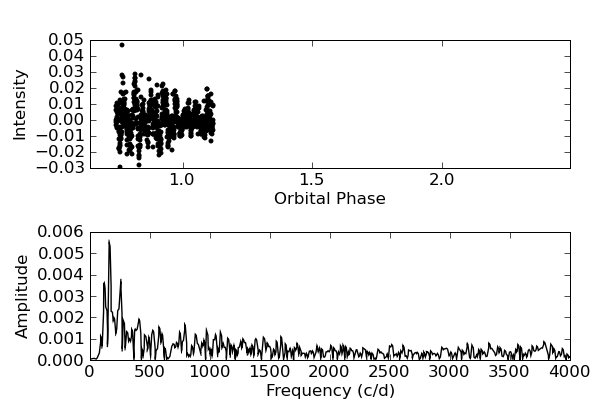
\includegraphics[width = 0.50\columnwidth, bb=0 0 600 400]{images/archive_phot/norm_int_eclipsing/S6555d_FF.png} &
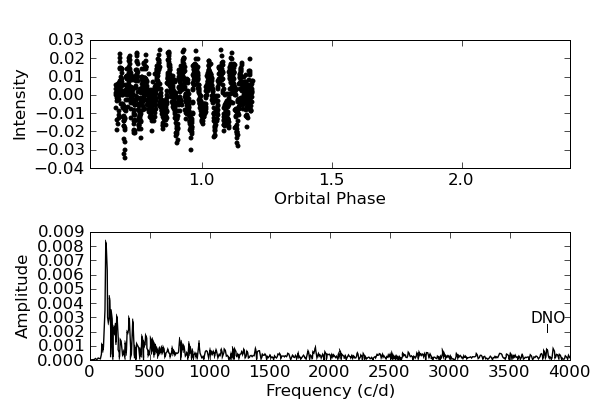
\includegraphics[width = 0.50\columnwidth, bb=0 0 600 400]{images/archive_phot/norm_int_eclipsing/S6564d_FF.png} \\
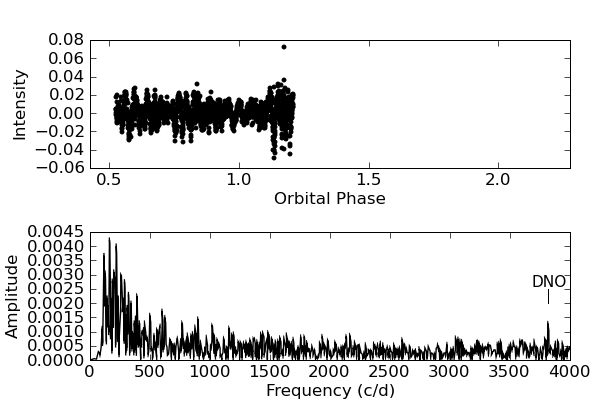
\includegraphics[width = 0.50\columnwidth, bb=0 0 600 400]{images/archive_phot/norm_int_eclipsing/S6570d_FF.png} &
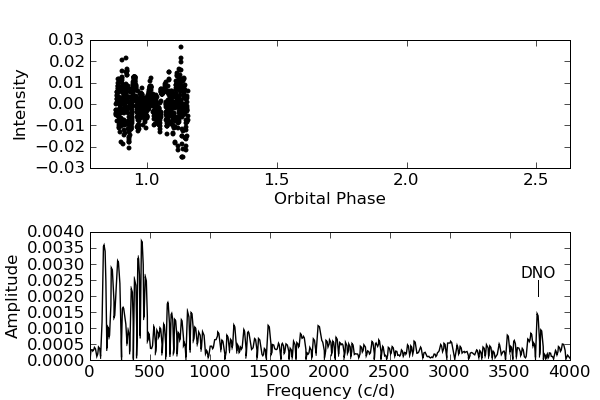
\includegraphics[width = 0.50\columnwidth, bb=0 0 600 400]{images/archive_phot/norm_int_eclipsing/S6660d_FF.png}

\end{tabular}
\end{narrow}
\caption[Flattened lightcurves and periodograms of EC2117-54.]{Flattened lightcurves and periodograms 
of EC2117-54. Clockwise from Top-left: Run S6544, S6548, S6551, S6564, S6660, S6570, S6555 and S6549.} 
\label{ec2117_archive}
\end{figure}


\begin{figure}
\begin{narrow}{-1in}{0in}


\begin{tabular}{cc}
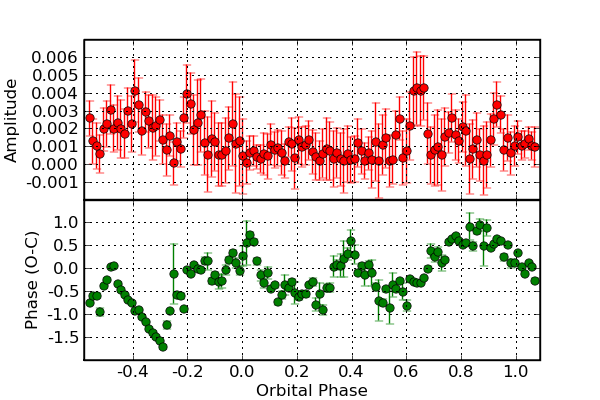
\includegraphics[width = 0.65\columnwidth, bb=0 0 600 400]{images/archive_phot/norm_int_eclipsing/S6544_23.13.png} &
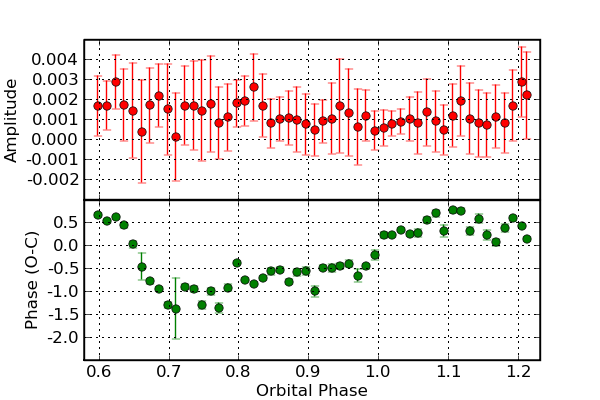
\includegraphics[width = 0.65\columnwidth, bb=0 0 600 400]{images/archive_phot/norm_int_eclipsing/S6549_22.60.png} \\
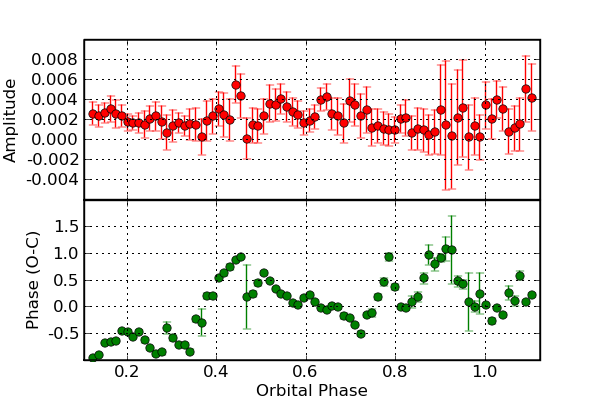
\includegraphics[width = 0.65\columnwidth, bb=0 0 600 400]{images/archive_phot/norm_int_eclipsing/S6551d_22.66.png} &
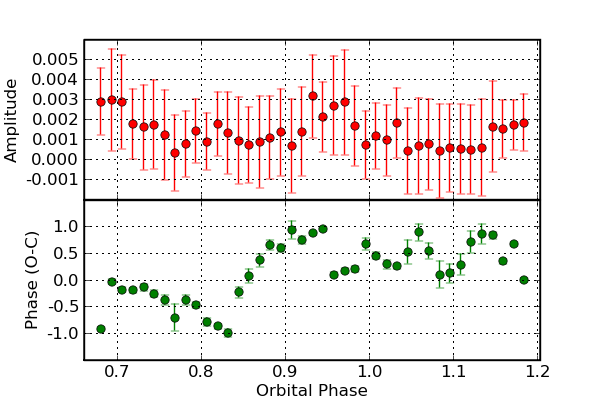
\includegraphics[width = 0.65\columnwidth, bb=0 0 600 400]{images/archive_phot/norm_int_eclipsing/S6564d_22.68.png} \\
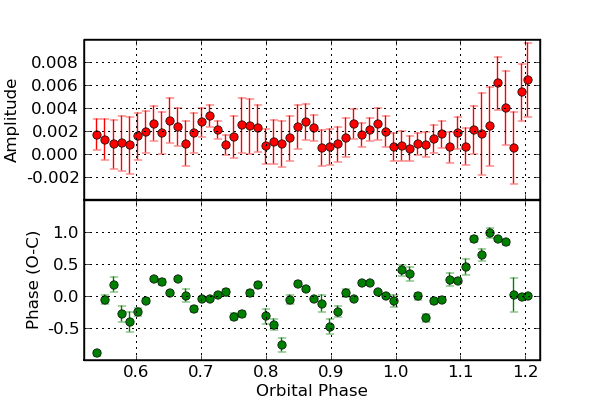
\includegraphics[width = 0.65\columnwidth, bb=0 0 600 400]{images/archive_phot/norm_int_eclipsing/S6570_22.63.png} &
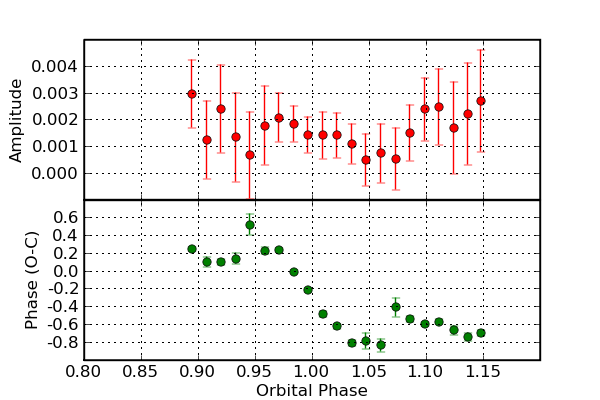
\includegraphics[width = 0.65\columnwidth, bb=0 0 600 400]{images/archive_phot/norm_int_eclipsing/S6660d_FF_OC.png} 
\end{tabular}
\end{narrow}
\caption[$O-C$ diagrams of DNOs in archive data.]{$O-C$ diagrams of DNOs in archive data. Clockwise from top left: Run S6544, S6549, S6564, S6551, S6660, S6570. All diagrams were calculated using 15 cycles with 50\% overlap. Phase panels were calculated relative to constant signals with periods as listed in Tab. \ref{RO_table}.} 
\label{ec2117_archive_OC}


\end{figure}






\chapter{Spectroscopy of EC2117-54}

\section{Observations}
\subsection{Southern African Large Telescope}
\label{SALT}

The Southern African Large Telscope (SALT) is the newest addition to the collection of telescopes operated by the South African Astronomical Observatory (SAAO). Construction has recently been completed and, although the telescope is currently in its performance verification stage, it has already produced its first scientific results \citep{salt_first_science}.

This telescope is the largest single telescope in the southern hemisphere. Its design is based on the Hobby-Eberly Telescope (HET) situated at the McDonald Observatory in Texas. The unique design of these telescopes allows for large telescopes to be built at a fraction of the cost of conventional Altitude-Azimuth (Alt-Az) telescopes. 

The telescope is unconventional in that its instruments are installed in a moving structure called the \texttt{Tracker}. The tracker moves the instruments along a theoretical surface that is concentric with the spherical surface of the main mirror. Therefore in principle it works in a similar fashion to the Arecibo radio telescope. The tracker is located at a distance of $13.08 \hspace{2pt}m$ from the primary mirror, which is half the radius of curvature. Because the primary mirror is spherical, the tracker houses a Spherical Aberration Corrector (SAC) \citep{dod2000}.

The main mirror consists of 91 hexagonal mirrors made of Astro-Sitall \citep{swiegers}. Each mirror is supported by  actuators. These are used to tip-tilt corrections of the individual mirror segments. The individual segments are also also fitted with capacitive edge sensors which are used to detect changes in the position of the individual mirrors. The changes can then be corrected. During observation, this is done at $20s$ intervals.

The primary mirror is supported by a steel structure which fixes the altitude at which the telescope points at  $37^{\circ}$. The telescope can only move in azimuth. The telescope can therefore only point to objects in an annulus in the sky at any particular moment. To observe targets outside the annulus, the operators will have to wait for these objects to move into the annulus. Objects can generally be observed twice in an evening. If the objects happen to move across the northern or southern regions of the annulus, they can be observed for longer periods ($\approx$ 4 hours) than when they move overhead from East to West ($\approx $ 1 hour on each side). To observe an object, the telescope is moved to the appropriate azimuth. The tracker is then used to follow the object as it tracks across the primary mirror.




\subsection{Robert Stobie Spectrograph}
\label{RSS}

The Robert Stobie Spectrograph (RSS), previously known as the Prime Focus Imaging Spectrograph (PFIS) is, together with SALTICAM, one of the first-generation instruments on the Southern African Large Telescope (SALT). It is a multipurpose medium resolution spectrograph. Its capabilities include medium-band imaging, Fabry-Perot imaging, longslit and multislit grating spectroscopy. High time-resolution and polarimetric modes are also possible. \citep{RSS_Modes}

A full description of the operational modes of RSS is given by \cite{RSS_Modes}. The modes relevant to this project will be summarised here.

The instrument can be seen as 4 systems in series namely the focal plane system, the dispersive elements, polarization optics and the CCD detector.

The focal plane system can be used in \textit{open}, \textit{longslit} and \textit{slitmask} mode. In \textit{open} mode there is no slitmask allowing direct imaging of objects. The \textit{longslit} mode is the standard spectroscopic mode used by most spectrographs and is also the mode used for the August 2006 observations while the \textit{slitmask} mode uses a custom laser-cut slit for multi-object spectroscopy and spectropolarimetry. \citep{RSS_Modes}

The second subsystem, the dispersive elements, comprises of an \textit{imaging mode}, \textit{Fabry-Perot} imaging mode, and a \textit{grating spectroscopy} mode \citep{RSS_Modes}. The grating spectroscopy mode was used for the August 2006 observations.

The polarization optics subsystem allows various polarimetric observations to be made. This system was not used and will not be discussed further. See \cite{RSS_Modes} and the references therein for a complete overview of this system.

The detector of the RSS comprises of 3 Marconi Applied Technologies 44-82 CCDs, each with 2048x4096 pixels of size 15 microns. The CCDs are mosaiced to form a larger detector. Each CCD has 2 amplifiers to decrease readout times. The plate scale at the detector is 117 microns/arcsec and will therefore mostly be used with 2x2 binning in order to reduce readout noise. The CCDs can be operated in 3 different modes. These are \textit{normal}, \textit{fast} and \textit{charge shuffle} modes. The \textit{normal} mode allows the entire mosaic to be read in 3.6s using 2x2 binning with 5e/pix noise \citep{RSS_Modes}. Using the frame transfer capability of the \textit{fast} readout mode, images can be obtained 1.8s apart. This is the mode used in the August 2006 observations. 


During the August 2006 observations, the telescope was still in its performance verification phase and the design specifications of RSS have not yet been met. As a result, the operation modes listed by \cite{RSS_Modes} and \cite{RSS_Opt_Design} could not be used and less than optimal observations were obtained.






\subsection{Spectroscopic observations in 2006}
\label{obs_spec}


Spectroscopic observations of EC2117-54 were made on the night of 17 August 2006 (JD 2453965) using the Robert Stobie Spectrograph (Section \ref{RSS}) by Encarni Romero-Colmenero, the on-duty SALT astronomer. A total of 335 exposures were obtained of the object as it went through eclipse. An integration time of 5s were used in order to fully sample possible lpDNOs and possibly DNOs that may occur during this time. A further $\sim5$s were needed to read out the CCDs which results in $\sim10.5$s between exposure start times. A pre-binning of 2x2 was used together with the ``bright'' gain setting, grating 0900 and a grating angle of $14.38^{\circ}$. The gain for each CCD was manually modified to avoid discontinuities in the spectra between CCDs. This is explained in Section \ref{calibrate}. A slit-width of $1.5''$ was used to minimise slit-losses. Spectra of an CuAr calibration lamp were obtained before and after the run to allow wavelength calibration and to correct for any time-dependent shifts in the instrument. The spectra obtained have a resolution of $\sim$ 0.94\AA{} over the wavelength range 3933.8\AA{} - 7022.1 \AA{}.

A spectrophotometric standard star was observed using the same instrument setup for flux calibration purposes. Absolute flux-calibration is however not possible with SALT due to the varying aperture size. These observations will only allow the shape of the spectrum to be corrected. The flux was calibrated using the middle CCD, covering the wavelength range of a Johnson V-band filter, and the simultaneous photometric observations. 

\begin{figure}
 \centering
 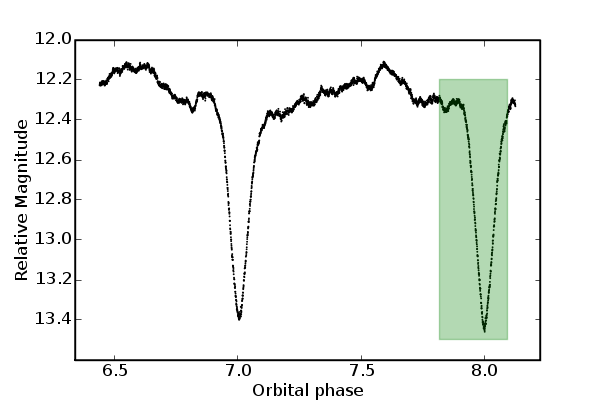
\includegraphics[width=0.9\columnwidth,bb=0 0 600 400]{images/S7655_SALT_coverage.png}
 % S7655_SALT_coverage.png: 600x400 pixel, 72dpi, 21.17x14.11 cm, bb=0 0 600 400
 \caption[Simultaneous photometry and spectroscopy]{The lightcurve of the photometric run S7655 and the simultaneous coverage of SALT high-speed spectroscopy (shaded area).}
 \label{spec_SALT_coverage}
\end{figure}




\section{Reductions}
% \subsection{Reduction of Spectroscopic Observations}
% \label{spec_reduce}

The Robert Stobie Spectrograph (RSS) is the first-generation spectrograph fitted to the SALT. It was previously known as the Prime Focus Imaging Spectrograph (PFIS). It is a medium resolution spectrograph with 3 CCD detectors. Each CCD has 2 amplifiers in order to reduce the readout time. A raw SALT RSS FITS file therefore consists of six data blocks and a single header block. In order to extract a spectrum from an image, it is necessary to perform a number of initial operations on the raw FITS file to get the data in a usable form. 

It was decided to perform the spectroscopic reductions separately on each CCD. Knowledge of the relative positions and rotations between the CCDs would therefore not be needed. Each CCD image was separately mosaiced, calibrated, extracted and wavelength calibrated. The three resulting spectra were then joined to form a single spectrum. These steps are outlined below.

The preparation of the images were performed using a script written by the author in the \texttt{Python} language. An example of it can be seen in Section \ref{pysalt}. 

\subsection{Mosaicing and Calibration}
\label{calibrate}

Each CCD has 2 amplifiers which will generally have different nominal gain settings at the time the image is read from the CCD device. The different amplifiers will therefore need to be gain-corrected separately, each with its own gain value. It was found that using the gain values specified in the FITS header resulted in an extracted spectrum that exhibited discontinuities across the boundary between different amplifiers, as well as between adjacent CCDs. This problem was fixed by calculating the median value of pixels on either side of each boundary and calculating a multiplication factor that would allow the extracted spectrum to be continuous across these boundaries. The gain factors did not need to be absolute since the extracted spectra were later flux calibrated using observations of a spectrophotometric standard star.

Each CCD was then bias-corrected using the overscan region. The median value of the overscan region was calculated and subtracted from the CCD image.

The mosaicing of these CCD images was trivial since they do not overlap. The size of the resulting image was known \textit{a priori}. A new empty image was created with dimensions $(R,2C+1)$ where $R$ is number of rows and $C$ is number of columns of each amplifier region. The two amplifier images were then added to the empty image in their correct place. The extra column inserted is the boundary between adjacent amplifiers. This empty column was filled by replacing every empty pixel by the average value of its two adjacent pixels. The bad column on CCD no. 1 was also corrected in this fashion.

Since the flatfield images had a number of saturated pixels, the spectroscopic images could not be corrected for pixel to pixel variations.

The resulting calibrated and mosaiced images were then written to disk in a new FITS file. Selected header entries copied from the primary header unit were added to each output file.

These steps were performed automatically on all raw files using the script shown in Section \ref{pysalt}.


\subsection{Spectrum Extraction}
\label{specextract}

The next step in the reduction process was to obtain wavelength- and flux-calibrated spectra from the prepared images. The extraction was done using the \texttt{IRAF} package. It was found that automating complex reductions of this nature is made difficult when using the scripting facilities in standard \texttt{IRAF}\footnote{IRAF is distributed by the National Optical Astronomy Observatory, which is operated by the Association of Universities for Research in Astronomy, Inc., under cooperative agreement with the NSF.}. Instead, \texttt{Pyraf} scripts were used to automate the spectrum extraction process. The steps followed were obtained from \cite{slitspecIRAF}.

In order to automate the reduction process, an example reduction was made manually to model subsequent reductions on. Since it was decided to separately extract and wavelength calibrate each CCD, 3 manual extractions were made for the EC2117-54 images. There was only a single exposure obtained for EG21, the spectrophotometric standard star. The extraction process for these images was completed manually using the \texttt{apall} task in \texttt{IRAF}.

The steps needed to extract an exposure are as follows:

\begin{itemize}
 \item Locate spectrum on image
 \item Trace spectrum
 \item Specifying spectrum and background windows
 \item Extraction using optimal method
 \item Extracting calibration arcs
 \item Identifying calibration arc lines and wavelength calibration
\end{itemize}

These steps were completed manually for the first exposures on each CCD. The object and background windows were specified in the interactive window of the \texttt{apall} task.

The second step, tracing the spectrum, is the process of finding the center of the object spectrum along the dispersion direction. This is necessary because any misalignment in the spectrograph, as well as the differential atmospheric refraction for different wavelengths, can cause the spectrum to not be perfectly aligned with the pixel rows on the CCD. The image columns are summed along the dispersion direction in multiple steps. For each summed column, the row number of the peak is found. The peak positions as a function of column number is then fitted with a polynomial. This function  then defines the center of the spectrum in subsequent reductions.

At this point the spectrum can be extracted from the image. The \texttt{apall} task was used for this purpose. It allows different extraction algorithms to be used. The ``Optimal'' algorithm was used to extract all the spectra. This algorithm weights every pixel according to its noise characteristics. It takes into account Poisson and readout noise. Therefore, pixels with a high signal-to-noise (S/N) ratio will be given more weight. This reduces the amount of noise in the extracted spectrum that is caused by pixels with low S/N. The details of this algorithm are given in \cite{HorneOpt}.

The calibration arcs were extracted using the same extraction window as for the object spectra. Calibration arcs of a CuAr lamp were observed before and after the run. These were used to correct for any linear shift in the instrument that may have ocurred during the observations. In order to obtain a wavelength scale for every pixel, a spline is fit to a wavelength versus pixel number plot where the wavelengths are obtained from fits to emission lines in the calibration spectra. I verified that the RMS error of the wavelength solution is $\sim 0.3$ for each spectrum. The wavelength calibration was done using the \texttt{identify} task in \texttt{IRAF}.

Subsequent exposures were extracted by using the first spectrum as starting point and then refitting the trace. The reductions were done by using the \texttt{Python} script in Appendix \ref{spec_extr}.


\subsection{Spectrum Calibration}
\label{spec_cal}

The extracted spectra now needs to be wavelength and flux-calibrated. The wavelength calibration process was done using the \texttt{identify} task in \texttt{IRAF}. This was done for a single arc spectrum. The subsequent arc spectra were wavelength-calibrated using the \texttt{reidentify} task. These tasks calculated the dispersion solution for each exposure, which were then applied to the object spectra using the \texttt{dispcor} task.

The flux calibration was based upon the spectrum of the spectrophotometric standard star, EG21 \citep{1984MNRAS.206..241B}. The sensitivity function was calculated using the \texttt{sensfunc} task and was applied to all off the EC2117-54 spectra using the \texttt{calibrate} task. Figure \ref{cal_uncal} displays the spectrum of EG21 before and after calibration.

Due to the changing pupil size of SALT, absolute flux calibration is not possible. It was decided to use the V-band photometry obtained using the SAAO 1.9m to correct for the effects of the changing pupil size. The photometric lightcurve was transformed from magnitude to intensity and was normalised by its mean. Its smoothed version, obtained from the flattening process, was used to calculate the correction. Firstly, the intensity values at the times of the spectroscopic exposures was interpolated. Then, for each of the spectroscpic exposures, the ratio of the photometric intensity and the sum of the middle CCD was calculated. This value transforms the spectroscopic flux to intensity. This value was then applied to the entire spectrum. The process is then repeated for every spectroscopic exposure.


\subsection{Signal-to-noise}
\label{signaltonoise}
The signal-to-noise (S/N) was calculated for every spectrum using the \texttt{splot} command in IRAF. Continuum regions with no detectable emission or absorption were chosen from which to calulate the S/N. The regions 6350\AA--6450\AA, 5474\AA--5574\AA\hspace{2pt} and 4450\AA--4550\AA\hspace{2pt} were chosen for the red, yellow and blue regions of the spectrum respectively. Figure \ref{snr} shows the calculated S/N as a function of orbital phase. The S/N for the blue end is significantly lower than for the red end, even though a much higher flux is expected from the blue end. At the end of the observing run, the S/N is lower than at the start. This is due to the reduction of SALT pupil size during the observations which caused an increasingly smaller amount of light to be observed thereby reducing the S/N.

In order to judge the quality of the observations, the expected S/N was calculated using the observation planning tool that is available from the SALT website\footnote{http://www.salt.ac.za/proposing/observation-planning-tools/}. The S/N was calculated for the telescope configuration at the time of the observations for a point source with magnitude V=14.7 and V=13.7 which correspond to EC2117-54 in and out of eclipse respectively. The expected S/N was calculated to be 31 for V=14.7 and 59 for V=13.7. The measured S/N of the observations is significantly lower than expected. This signal degradation was mainly caused by a seal that started leaking fluid, which in turn caused a chemical reaction in a lens, reducing its transparency severely. Measurements of the throughput suggests that the spectrograph have nominal throughput at 8000\AA, $\sim35$\% deficiency at 5500\AA \hspace{2pt} and $\sim50$\% deficiency at 4300\AA \hspace{2pt} (O'Donoghue, 2006, private communication). 

\begin{figure}
\centering
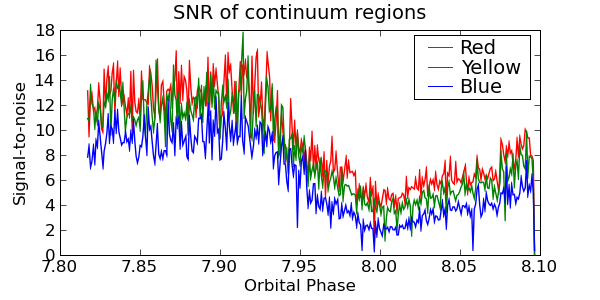
\includegraphics[width=0.8\columnwidth, bb=0 0 600 300]{spectroscopy/snr/continuum_snr.png}
\caption[Signal-to-noise curves]{Signal-to-noise (S/N) ratio as a function of orbital phase. The regions used for calculating the S/N are, Red (6350\AA--6450\AA), Yellow (5474\AA--5574\AA), Blue (4450\AA--4550\AA). } 
\label{snr}
\end{figure}


%##################################################################################################################################33

\begin{figure}
\begin{narrow}{-1in}{0in}
\begin{tabular}{cc}
 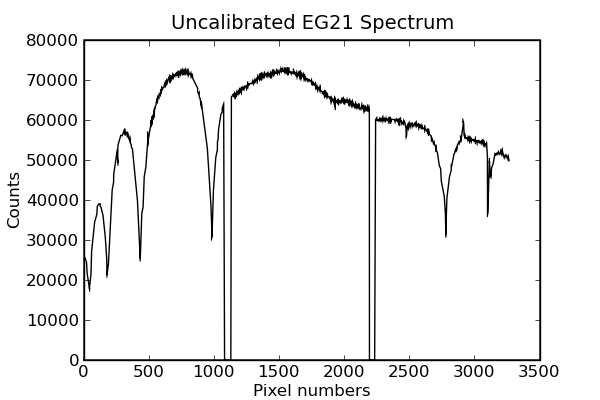
\includegraphics[width=0.65\columnwidth, bb=0 0 600 400]{images/uncalEG21.png} &
 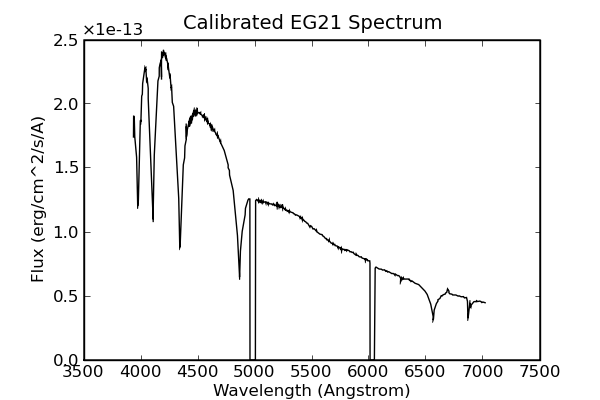
\includegraphics[width=0.65\columnwidth, bb=0 0 600 400]{images/calEG21.png} \\
\end{tabular}
\end{narrow}
\caption[EG21 spectrum before and after flux-calibration]{EG21 spectrum before and after flux- and wavelength-calibration} 
\label{cal_uncal}

\end{figure}

%##################################################################################################################################33

% \pagebreak


\pagebreak
\section{Analysis}
\label{spec_analysis}


\begin{figure}
\centering
\begin{narrow}{-1in}{0in}
 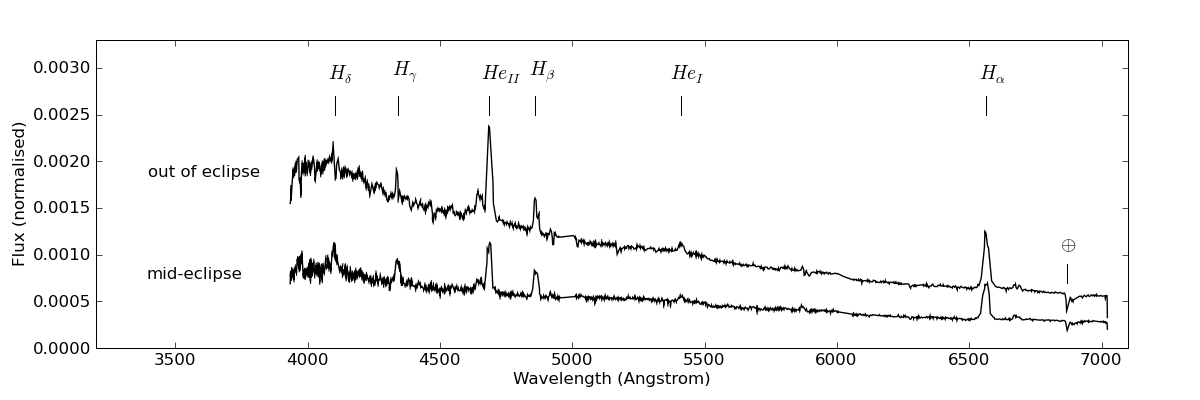
\includegraphics[width=1.4\columnwidth,bb=0 0 1200 400]{spectroscopy/spec_properties/in_out_eclipse.png}
 % in_out_eclipse.png: 1200x400 pixel, 100dpi, 30.48x10.16 cm, bb=0 0 1200 400
 
\end{narrow}
\caption[Average out-of-eclipse and mid-eclipse spectra of EC2117-54]{Average out-of-eclipse and mid-eclipse spectra of EC2117-54. The average spectrum of EC2117-54 shows broad Balmer, He I and He II lines. The out-of-eclipse spectrum (top) was obtained by averaging all spectra between orbital phases 7.817 and 7.9. During mid-eclipse (orbital phase $7.95 < \phi < 8.05$) the continuum is flatter and the He II line is comparatively weaker. The position of prominent lines and a terrestrial feature have been marked.}
\label{average_spec}
\end{figure}

%##################################################################################################################################33

\begin{figure}
\begin{narrow}{-1.2in}{0in}
 \centering
 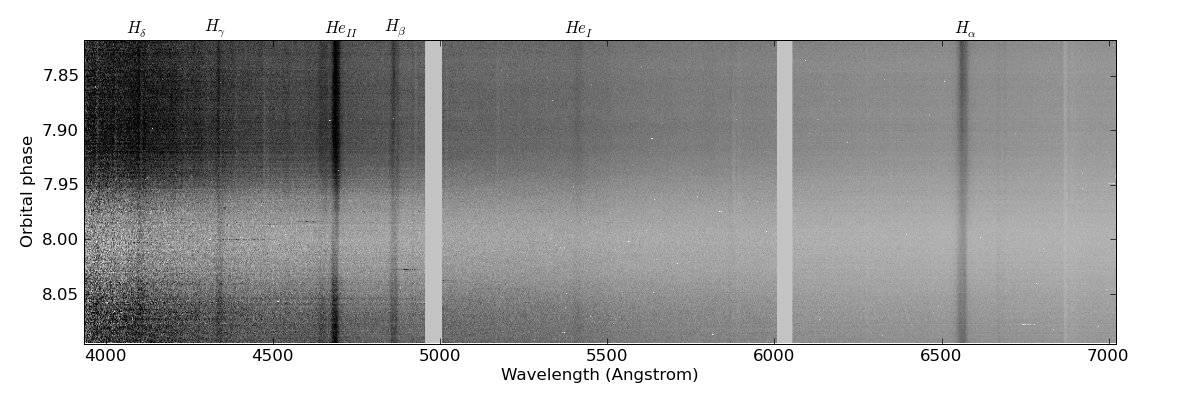
\includegraphics[width=1.5\columnwidth,bb=0 0 1200 400]{spectroscopy/final/specgram_full.png}
 % specgramHa.png: 1179666x1179666 pixel, 0dpi, infxinf cm, bb=
\end{narrow}
 \caption[Trailed spectrum for the entire spectroscopic run.]{Trailed spectrum for the entire spectroscopic run. Grayscale denotes flux level (Darker$=$higher). Important emission lines have been labelled.  }
 \label{specgram_full}
\end{figure}

%##################################################################################################################################33




\subsection{Spectral Properties}
\label{spectral_prop}

Figure \ref{average_spec} shows the average spectra of EC2117-54 in eclipse and out of eclipse. The out-of-eclipse spectrum shows broad double-peaked Balmer ($H_{\alpha}$ and $H_{\beta}$) emission and a strong He II line at 4686\AA{}. The spectra are very noisy for wavelengths bluer than $\sim5000$\AA{}. This was caused by faulty optics in the RSS that have since been repaired. This caused the higher order Balmer lines and the He II line to have a lower than expected S/N ratio. The blueshifted peaks of the Balmer lines are stronger than the redshifted peaks. This effect has been observed in other cataclysmic variables. \cite{V2051Oph2001} noted this effect in V2051 Oph but did not attempt an interpretation, other than the blue side of the accretion disk making a larger contribution to the emission. The continuum shows a steep slope towards shorter wavelengths, revealing the presence of a very hot central component in the system. The out-of-eclipse spectrum was obtained by averaging all spectra up to orbital phase 7.9.  The mid-eclipse spectrum (bottom spectrum Fig. \ref{average_spec}) was calculated by averaging the spectra between orbital phases 7.95 and 8.05. This spectrum has a flatter continuum than the out-of-eclipse spectrum.  This shows that the secondary star is cooler than the primary star and the inner regions of the accretion disk. During eclipse it contributes a greater fraction of the total light, causing a reddening of the spectrum.

% \textbf{Add some stuff about the trailed spectrograms.}









%##################################################################################################################################33

\begin{figure}
 \centering
 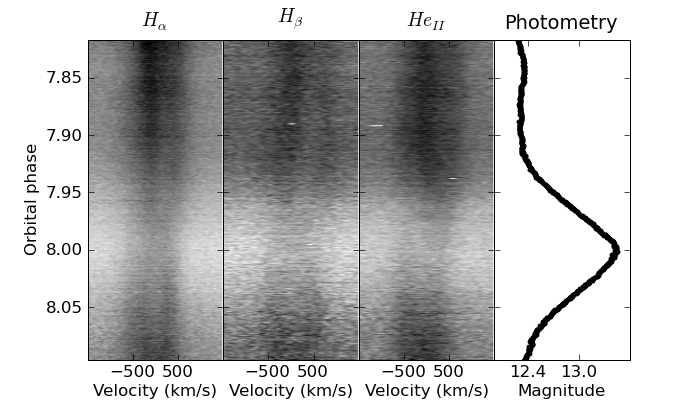
\includegraphics[width = \columnwidth, bb=0 0 700 400]{spectroscopy/final/specgram.png}
 % specgramHa.png: 1179666x1179666 pixel, 0dpi, infxinf cm, bb=
 \caption{Trailed spectrum around the $H_{\alpha}$,$H_{\beta}$ and $He_{II}$ lines.}
 \label{specgram}
\end{figure}

%##################################################################################################################################33




% %##################################################################################################################################33
% 
% \begin{figure}
% \centering
% \begin{narrow}{-1in}{0in}
% \begin{tabular}{cc}
% 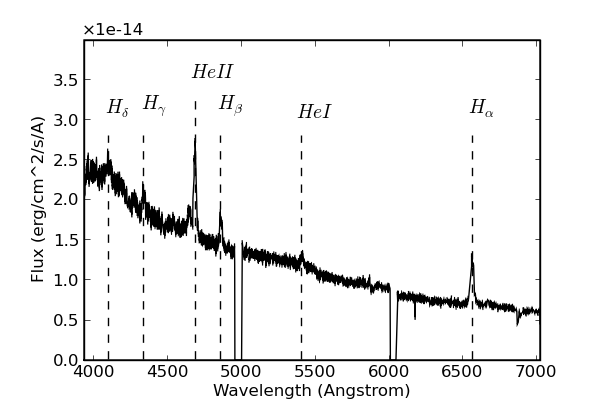
\includegraphics[width=0.65\columnwidth, bb=0 0 600 400]{images/EC2117.png} & 
% \includegraphics[width=0.65\columnwidth, bb=0 0 600 400]{images/EC0010.png} \\
% \end{tabular}
% \end{narrow}
% \caption[Single and average EC2117-54 spectra]{Left: Average EC2117-54 spectrum. Right: Single EC2117-54 spectrum. Important emission lines have been labelled.} 
% \label{EC2117ave_single}
% \end{figure}
% 
% %##################################################################################################################################33



\subsection{Time Variability}
\label{spec_timevar}

In order to study rapid time variability in the optical spectrum of EC2117-54, a number of different methods were investigated. Each spectrum was summed over all wavelengths to construct a lightcurve. The lightcurve was normalised by dividing by the mean. The periodogram of this lightcurve was inspected, but did not show any evidence for the periodicities seen in the photometric lightcurve. This suggests that the S/N ratio of the spectroscopic observations are significantly lower than the photometric observations. 
\begin{figure}[t]
 \centering
 \includegraphics[width=\columnwidth,bb=0 0 800 600]{spectroscopy/lightcurves/eq_wid_lc.png}
 % eq_wid_lc.png: 800x600 pixel, 100dpi, 20.32x15.24 cm, bb=0 0 600 400
 
 \caption[Equivalent width time-series]{The equivalent width of the $H_{\alpha}$, $H_{\beta}$ and $He_{II}$ lines as a function of orbital phase (top panel) and the corresponding periodograms (bottom panels).}
\label{eq_width_lc}
\end{figure}
The equivalent width of the three most prominent lines were measured for every spectrum using the \texttt{splot} task of the \texttt{IRAF} suite. Figure \ref{eq_width_lc} shows the equivalenth width of the $H_{\alpha}$, $H_{\beta}$ and $He_{II}$ lines as a function of orbital phase and the corresponding periodograms. The Balmer lines become wider through eclipse but the He II line does not. This can be explained by examining the trailed spectrum in Fig. \ref{specgram}. The Balmer lines can be seen to have stronger emission outside eclipse. They have strong blueshifted components and  weaker redshifted components. The reason for this is unclear. During eclipse the Balmer lines become weaker but have an increased equivalent width. This was also seen in the SW Sex star, HS 0728+6738, by \cite{2004A&A...424..647R}. The equivalent width increases because the continuum source is eclipsed to a greater degree than the emission line source, suggesting that the Balmer emission originates from an optically thin region above the accretion disk. The He II line behaves differently. It stays mostly uneclipsed until $\sim$7.95 where it starts to be eclipsed. The blueshifted component is eclipsed first, as is expected from a progradely orbiting source. The fact that the ionised helium emission is nearly totally eclipsed and the eclipse duration is very short, suggests an origin in the inner regions of the accretion disk. The equivalent width curve of the He II line (Fig. \ref{eq_width_lc}) also supports this hypothesis. The equivalent width is nearly constant throughout the eclipse. The He II emission is expected to originate close to the centre of the system because the formation of higher excitation lines of helium require high temperatures. 

The possible signals detected in the periodograms in Fig. \ref{eq_width_lc} were compared to those obtained from the photometric observations. The peaks in the periodograms do not correspond to any known periodicity detected during this or previous studies of the system. The spectra were then phase-folded on all possible periods detected during this study. Because the DNOs and lpDNOs are thought to originate from rapidly rotating bright regions, a modulation that moves from the blue side of the emission lines to the red side are expected. It is assumed the bright regions rotate in a prograde direction. Folding the spectra on the oscillation period should therefore result in a diagram that shows a bright region that moves sinusoidally from the blue to red on an image that displays oscillation phase versus velocity (or equivalently, wavelength). An example of modulations in emission lines in the system V2051 Oph can be seen in Fig. 7 and Fig. 8 of \cite{V2051Oph2001}. 

Because the observations were done during the PV phase of SALT, the readout times were relatively long and low time resolution was obtained. For this reason, coupled with the throughput problems (see Section \ref{signaltonoise}), the folded spectra were averaged in 5 and 10 bins equally wide in phase space for the DNO (23.76s) and lpDNO (104.2s) signals respectively. Each bin was verified to contain approximately the same amount of spectra. No modulation at the DNO (23.76s) or lpDNO (104.2s) period is seen for any of the prominent lines. The process was repeated for all the possible periods obtained from the equivalent width curves, as well as from a lightcurve obtained by summing each full spectrum as well as each average-subtracted spectra. These are shown in the left panel of Fig. \ref{specgram_fold_ave_subDNO} and Fig. \ref{specgram_fold_ave_sublpDNO}. No evidence for modulation of the line profiles at the periods detected in the photometric lightcurves were detected. As a check, the spectra were folded on a period of 25s.  The right panel of Fig. \ref{specgram_fold_ave_subDNO} displays this plot. This plot is nearly identical to the left panel of Fig. \ref{specgram_fold_ave_subDNO} even though there are no signals detected with a period of 25s in either the photometry or the spectroscopy. This casts doubt on any systematic variations that may be seen in Fig. \ref{specgram_fold_ave_subDNO} and Fig. \ref{specgram_fold_ave_sublpDNO}. The absence of modulations in the phase-folded spectra suggests that the phase-folded spectra contain only noise and that the S/N ratio of the spectroscopic observations are indeed too low to detect the DNOs and lpDNOs or that the line modulation seen in V2051 Oph \citep{V2051Oph2001} is not present in EC2117-54.

The phase folded spectra were created from spectra at orbital phases less than 7.9. Figure \ref{snr} shows this region to have relatively high S/N (S/N $\geq$10) and therefore should show some evidence of line modulations if they are present. Contrary to this is the absence of DNOs in equivalent-width curves and lightcurves created from the spectroscopic data, suggesting that the S/N was indeed too low and that the absence of detected modulations is due to this. Although it is surprising that the spectra did not contain any evidence of rapid oscillations, it is not surprising that EC2117-54 behaves differently from V2051 Oph. V2051 Oph is classified as an SU UMa star where EC2117-54 is a nova-like. They lie on opposite sides of the period-gap and probably have very different mass-transfer rates and hence accretion disk structure. In short, there is much difference between the two systems.

\begin{figure}[ht]
\begin{narrow}{-1.25in}{0in}
\begin{tabular}{cc}
\includegraphics[width=0.7\columnwidth, bb = 0 0 1200 600]{spectroscopy/final/specgram_fold_ave_sub_DNO23.76.png} & 
\includegraphics[width=0.7\columnwidth, bb = 0 0 1200 600]{spectroscopy/final/specgram_fold_ave_sub_DNO25.0.png}
 % specgram_fold_23.76.png: 1179666x1179666 pixel, 0dpi, infxinf cm, bb=
\end{tabular}
\end{narrow} 

\caption[Average-subtracted spectra folded on DNO period]{Average-subtracted spectra folded on DNO (23.76s) period (left panel) and mock (25.0s) period (right panel). The two plots look very similar and suggests that any no modulations can be detected at the DNO period. Black represents emission.}
\label{specgram_fold_ave_subDNO}
\end{figure}

% \begin{figure}
% \begin{narrow}{-0.in}{0in}
% \centering
%  \includegraphics[width=1.0\columnwidth, bb = 0 0 1200 600]{spectroscopy/final/specgram_fold_ave_sub_DNO25.0.png}
%  % specgram_fold_23.76.png: 1179666x1179666 pixel, 0dpi, infxinf cm, bb=
% \end{narrow} 
% \caption[Average-subtracted spectra folded on DNO period]{Average-subtracted spectra folded on mock period (25.0s). Black represents emission. This plot was created to serve as a sanity-test.}
% \label{specgram_fold_ave_sub_sanity}
% \end{figure}

\begin{figure}[t]
\begin{narrow}{-0.in}{0in}
\centering
 \includegraphics[width=0.7\columnwidth, bb = 0 0 1200 600]{spectroscopy/final/specgram_fold_ave_sub_lpDNO104.2.png}
 % specgram_fold_23.76.png: 1179666x1179666 pixel, 0dpi, infxinf cm, bb=
\end{narrow} 
\caption[Average-subtracted spectra folded on lpDNO period]{Average-subtracted spectra folded on lpDNO (104.2s) period. Black represents emission.}
\label{specgram_fold_ave_sublpDNO}
\end{figure}
 

% \begin{figure}
%  \centering
%  \includegraphics[width=0.8\columnwidth,bb=0 0 600 400]{spectroscopy/lightcurves/fluxlightcurve.png}
%  % fluxlightcurve.png: 600x400 pixel, 100dpi, 15.24x10.16 cm, bb=0 0 600 400
%  \caption{Lightcurve of EC2117-54 obtained from spectroscopic run}
%  \label{speclightcurve}
% \end{figure}












%##################################################################################################################################33

% \begin{figure}
% \begin{narrow}{-1in}{0in}
% \begin{tabular}{lr}
%  \includegraphics[width = 0.65\columnwidth, bb=0 0 600 400]{images/vel_gauss.png} &
%  \includegraphics[width = 0.65\columnwidth, bb=0 0 600 400]{images/vel_ew.png} \\
%  \includegraphics[width = 0.65\columnwidth, bb=0 0 600 400]{images/lw_gauss.png} &
%  \includegraphics[width = 0.65\columnwidth, bb=0 0 600 400]{images/lw_ew.png}
% \end{tabular}
% \caption[Linewidths and velocities]{Linewidths and velocities} 
% \label{widths_velocities}
% \end{narrow}
% \end{figure}

%##################################################################################################################################33




%##################################################################################################################################33

% \begin{figure}
%  \centering
%  \includegraphics[width=0.9\columnwidth,bb=0 0 600 400 ]{images/ha_deblend.png}
%  % ha_deblend.png: 600x400 pixel, 72dpi, 21.17x14.11 cm, bb=0 0 600 400
%  \caption{$H_{\alpha}$ line deblended using double gaussian fit}
%  \label{ha_deblend}
% \end{figure}
% 
% \begin{figure}
%  \centering
%  \includegraphics[width=0.9\columnwidth,bb=0 0 600 400 ]{images/hb_deblend.png}
%  % ha_deblend.png: 600x400 pixel, 72dpi, 21.17x14.11 cm, bb=0 0 600 400
%  \caption{$H_{\beta}$ line deblended using double gaussian fit}
%  \label{hb_deblend}
% \end{figure}

%##################################################################################################################################33


% \begin{figure}
% \begin{narrow}{-0.8in}{0in}
% \centering
%  \includegraphics[width=1.2\columnwidth, bb = 0 0 1200 600]{spectroscopy/final/specgram_fold_23.76.png}
%  % specgram_fold_23.76.png: 1179666x1179666 pixel, 0dpi, infxinf cm, bb=
% \end{narrow} 
% \caption[Spectra folded on DNO period]{Spectra folded on DNO (23.76s) period. Black represents emission.}
% \label{specgram_fold_DNO}
% \end{figure}
% 
% \begin{figure}
% \begin{narrow}{-0.8in}{0in}
% \centering
%  \includegraphics[width=1.2\columnwidth, bb = 0 0 1200 600]{spectroscopy/final/specgram_fold_104.2.png}
%  % specgram_fold_23.76.png: 1179666x1179666 pixel, 0dpi, infxinf cm, bb=
% \end{narrow} 
% \caption[Spectra folded on lpDNO period]{Spectra folded on lpDNO (104.2s) period. Black represents emission.}
% \label{specgram_fold_lpDNO}
% \end{figure}






%\chapter{Analysis}

\section{Photometry}
\label{analysis_phot}

\subsection{Rapid Oscillations in photometric lightcurves}
\label{ro_phot_lc}
Photometry lightcurves from all 4 nights were flattened using the method described in section \ref{flat_section}. Periodograms were then calculated for these in order to identify any DNOs, lpDNOs and QPOs. Periodograms were calculated using the algorithm in \cite{kurtz_ft}. See figures \ref{S7651}, \ref{S7655} and \ref{S7659}. The DNO ($\sim3600$ cycles/day) and lpDNO($\sim1000$ cycles/day) spikes in the periodogram can clearly be seen in run S7651 and S7655. On the third night (Run \#S7659) the DNOs and lpDNOs were not visible. Run \# S7661 were hampered by cloud and only a very short observing run was possible. The data from this run were not used in any further analyses. The DNOs, lpDNOs and QPOs identified in the photometric lightcurves are shown in table \ref{RO_table}.

\begin{table}
\begin{scriptsize}
 
\centering
% use packages: array,supertabular
\begin{tabular}{ccccccc}
\hline \hline\\
Run    & DNO period & DNO freq      & lpDNO period & lpDNO freq     & QPO (s)\\ 
       & (s)        &  (cycles/day) &  (s)         &  (cycles/day)  &        \\ 
\\\hline \\
S7651  & 24.27, 24.15 & 3559.19, 3576.91 &  89.97 &  960.31  &  \\ 
S7655  & 23.76 & 3636.95 & 104.19 & 829.22 & \\ 
S7659  & --& --& -- &&\\ 
S7661  & -- & -- & -- &&\\\\
\hline
\end{tabular}

\caption[Rapid Oscillations in photometry]{Rapid Oscillations in photometry.}
\label{RO_table}
\end{scriptsize}
\end{table}



\subsubsection{Run S7651}

The periodogram of the flattened lightcurve of run S7651 (figure \ref{S7651}) shows evidence for a double DNO with periods of 24.27s and 24.15s (table \ref{RO_table}). The $O-C$ diagrams (figures \ref{OC_S7651_1} and \ref{OC_S7651_2} ) show evidence of DNOs with changing phases. Examining the spectrogram (figure \ref{trailed_ft_S7651}) for this run, the DNO seems to show only a single frequency. The resolution of the spectrogram is not high enough to discern these different DNOs since their periods are very similar (table \ref{RO_table}). The spectrogram shows a changing frequency of the DNO during eclipse. This is most probably due to a phase shift instead of a change in frequency of the actual oscillation.

There is evidence for an increase in the DNO amplitude in the $O-C$ diagrams and the spectrogram for this run. The same phenomenon is observed in run S7655, discussed in the following section.

The spectrogram was calculated from the flattened lightcurve of this run.



\begin{figure}
 \centering
 \includegraphics[width = 0.8\columnwidth, bb=0 0 600 400]{images/S7651.png}
 % vel_ew.png: 1179666x1179666 pixel, 0dpi, infxinf cm, bb=0 0 600 400
 \caption{Flattened lightcurve and periodogram for run S7651.}
 \label{S7651}
\end{figure}


\begin{figure}
 \centering
 \includegraphics[width = 0.8\columnwidth, bb=0 0 600 400]{images/run1_flat.png}
 % vel_ew.png: 1179666x1179666 pixel, 0dpi, infxinf cm, bb=0 0 600 400
 \caption[$O-C$ diagram of the 3559.19 cycles/day DNO of run S7651.]{$O-C$ diagram of the 3559.19 cycles/day DNO of run S7651. Diagram was calculated using 20 cycles with 50 \% overlap.}
 \label{OC_S7651_1}
\end{figure}


\begin{figure}
 \centering
 \includegraphics[width = 0.8\columnwidth, bb=0 0 600 400]{images/run1_flat_2.png}
 % vel_ew.png: 1179666x1179666 pixel, 0dpi, infxinf cm, bb=0 0 600 400
 \caption[$O-C$ diagram of the 3576.91 cycles/day DNO of run S7651.]{$O-C$ diagram of the 3576.91 cycles/day DNO of run S7651. Diagram was calculated using 20 cycles with 50 \% overlap.}
 \label{OC_S7651_2}
\end{figure}


\begin{figure}
 \centering
 \includegraphics[width = 0.8\columnwidth, bb=0 0 800 600]{images/trailed_FT_S7651_colour.png}
 % vel_ew.png: 1179666x1179666 pixel, 0dpi, infxinf cm, bb=0 0 600 400
 \caption[Raw lightcurve and spectrogram for run S7651.]{Raw lightcurve and spectrogram for run S7651. The spectrogam was calculated from the flattened lightcurve of this run using 600s segments with 50\% overlap.}
 \label{trailed_ft_S7651}
\end{figure}

\subsubsection{Run S7655}

The periodogram (figure \ref{S7655}) of the flattened lightcurve of this run shows a very strong peak at 3636.9 cycles/day (period of 23.8s). The $O-C$ diagram (figure \ref{OC_S7655}) supports a stable oscillation at this period. There is also a marked increase in the DNO amplitude near HJD $\sim0.41$ and $\sim0.57$ which is approximately the times of mid-eclipse. This notion is also supported by the spectrogram of this run (figure \ref{trailed_ft_S7655}). This amplitude increase is probably due to the decrease in non-oscillating light from the accretion disk during eclipse, which enables us to see the DNO source more clearly. The spectrogram shows the same ``frequency'' change seen in run S7651. This phase change can be seen in the $O-C$ diagrams that is concentrated on the times of eclipse (figures \ref{OC_S7655_eclipse1} and \ref{OC_S7655_eclipse2}).



The spectrogram was calculated from the flattened lightcurve of this run.



% $O-C$ diagrams (section \ref{ominc_section}) were calculated to track the changes in the DNOs, lpDNOs and QPOs. These are shown for run S7651 in figures \ref{OC_S7651_1} and \ref{OC_S7651_2} and for run S7655 in figure \ref{OC_S7655}.


\begin{figure}
 \centering
 \includegraphics[width = 0.8\columnwidth, bb=0 0 600 400]{images/S7655.png}
 % vel_ew.png: 1179666x1179666 pixel, 0dpi, infxinf cm, bb=0 0 600 400
 \caption{Flattened lightcurve and periodogram for run S7655.}
 \label{S7655}
\end{figure}

\begin{figure}
 \centering
 \includegraphics[width = 0.8\columnwidth, bb=0 0 600 400]{images/run2_flat.png}
 % vel_ew.png: 1179666x1179666 pixel, 0dpi, infxinf cm, bb=0 0 600 400
 \caption[$O-C$ diagram of the 3636.95 cycles/day DNO of run S7655.]{$O-C$ diagram of the 3636.95 cycles/day DNO of run S7655. Diagram was calculated using 20 cycles with 50 \% overlap.}
 \label{OC_S7655}
\end{figure}

\begin{figure}
 \centering
 \includegraphics[width = 0.8\columnwidth, bb=0 0 600 400]{images/run2_eclipse1_oc.png}
 % vel_ew.png: 1179666x1179666 pixel, 0dpi, infxinf cm, bb=0 0 600 400
 \caption[$O-C$ diagram first eclipse of the 3636.95 cycles/day DNO of run S7655.]{$O-C$ diagram first eclipse of the 3636.95 cycles/day DNO of run S7655. Diagram was calculated using 15 cycles with 50 \% overlap.}
 \label{OC_S7655_eclipse1}
\end{figure}

\begin{figure}
 \centering
 \includegraphics[width = 0.8\columnwidth, bb=0 0 600 400]{images/run2_eclipse2_oc.png}
 % vel_ew.png: 1179666x1179666 pixel, 0dpi, infxinf cm, bb=0 0 600 400
 \caption[$O-C$ diagram of the second eclipse of the 3636.95 cycles/day DNO of run S7655.]{$O-C$ diagram of the second eclipse of the 3636.95 cycles/day DNO of run S7655. Diagram was calculated using 15 cycles with 50 \% overlap.}
 \label{OC_S7655_eclipse2}
\end{figure}

\begin{figure}
 \centering
 \includegraphics[width = 0.8\columnwidth, bb=0 0 800 600]{images/trailed_FT_S7655_colour.png}
 % vel_ew.png: 1179666x1179666 pixel, 0dpi, infxinf cm, bb=0 0 600 400
 \caption[Raw lightcurve and spectrogram for run S7655.]{Raw lightcurve and spectrogram for run S7655. The spectrogam was calculated from the flattened lightcurve of this run using 600s segments with 50\% overlap.}
 \label{trailed_ft_S7655}
\end{figure}






\begin{figure}
 \centering
 \includegraphics[width = 0.8\columnwidth, bb=0 0 600 400]{images/S7659.png}
 % vel_ew.png: 1179666x1179666 pixel, 0dpi, infxinf cm, bb=0 0 600 400
 \caption{Flattened lightcurve and periodogram for run S7659.}
 \label{S7659}
\end{figure}




\section{Spectroscopy}

\begin{figure}
 \centering
 \includegraphics[width = 0.8\columnwidth, bb=0 0 600 400]{images/vel_gauss.png}
 % vel_ew.png: 1179666x1179666 pixel, 0dpi, infxinf cm, bb=0 0 600 400
 \caption{Line Velocities obtained by fitting gaussians.}
 \label{vel_gauss}
\end{figure}


\begin{figure}
 \centering
 \includegraphics[width = 0.8\columnwidth, bb=0 0 600 400]{images/vel_ew.png}
 % vel_ew.png: 1179666x1179666 pixel, 0dpi, infxinf cm, bb=0 0 600 400
 \caption{Line Velocities obtained using equivalent width measurements.}
 \label{vel_ew}
\end{figure}


\begin{figure}
 \centering
 \includegraphics[width = 0.8\columnwidth, bb=0 0 600 400]{images/lw_gauss.png}
 % vel_ew.png: 1179666x1179666 pixel, 0dpi, infxinf cm, bb=0 0 600 400
 \caption{Line widths obtained using fitted gaussians.}
 \label{lw_gauss}
\end{figure}


\begin{figure}
 \centering
 \includegraphics[width = 0.8\columnwidth, bb=0 0 600 400]{images/lw_ew.png}
 % vel_ew.png: 1179666x1179666 pixel, 0dpi, infxinf cm, bb=0 0 600 400
 \caption{Line widths obtained using equivalent width measurements.}
 \label{lw_ew}
\end{figure}



\begin{figure}
 \centering
 \includegraphics[width = \columnwidth, bb=0 0 800 800]{images/specgram.png}
 % specgramHa.png: 1179666x1179666 pixel, 0dpi, infxinf cm, bb=
 \caption{Trailed spectrogram around the $H_{\alpha}$,$H_{\beta}$ and \textit{HeII} lines.}
 \label{specgram}
\end{figure}






\chapter{Discussion}

\section{Photometry}
\label{photo_discussion}

Analysis of the August 2006 data for EC2117 reveals the presence of rapid oscillations. These are limited to DNOs and lpDNOs for the August 2006 dataset. The methods used to find and analyse rapid oscillations are not suitable to find QPOs. This is due to their low coherence and the fact that Fourier methods do not readily reveal the presence of non-stationary signals. More suitable methods do exist \citep{blackman}, but are outside the scope of this project. The lpDNOs do not show any systematic behaviour in the August 2006 photometric runs. They were only present in short sections of the lightcurves and could not be succesfully tracked through eclipse. Their point of origin in the system are therefore still unknown and the models suggested in \cite{DNOQPO_II} and \cite{DNOQPO_VI} cannot be tested using this dataset. 

The DNOs undergo different systematic phase changes through eclipse in multiple lightcurves. In run S7651, during the second eclipse (top-right panel of Fig. \ref{S7651_DNO}, and during the first eclipse of run S7655 (top-left panel of Fig. \ref{S7655_DNO}) it has a phase change similar to that of UX Uma (see Figure 7 in \cite{1980ApJ...241..247P}) where the phase changes by 1 cycle during eclipse. The DNO phase changes by $\sim$1 cycle before changing back to the phase that was present before the eclipse started in the first eclipse of run S7651 and second eclipse of run S7655. The same behaviour is seen in Z Cha during superoutburst in the middle panel of Fig. 10 in \cite{warner_brickhill}. These different scenarios are also encountered in EC2117-54 data retrieved from the archive.  There is also a smaller (shallower, faster) phase change before the aforementioned phase changes. 

The UX Uma-type phase change is explained in \cite{1980ApJ...241..247P} by a rotating-beam model. In this model it is assumed that the disk is axisymmetric; that the oscillation originates from a single spot on the equator of the white dwarf and that some the light from the emission spot is observed directly. The main variable parameter is the inclination of the system which is varied such that the white dwarf is not totally eclipsed. 

\cite{1980ApJ...241..247P} also simulates the phase change during eclipse of the 71s oscillation observed in DQ Her \citep{dqher} using a similar model to that of UX Uma. However, in the DQ Her model, the light from the emission spot is reprocessed and not seen directly. In this model, the phase change during eclipse is sinusoidal and highly dependent on the inclination of the system. Phase changes corresponding to different values for the system inclination are shown in Fig. 4 of \cite{1980ApJ...241..247P}. The sinusoidal curve predicted by the model for the phase change suggests that the Z Cha-type phase changes can be explained to some extent using this model. The idealised model from \cite{1980ApJ...241..247P} could perhaps be used to estimate the orbital inclination, however, this is outside the scope of this project and was not attempted.  The pre-eclipse phase change could possibly be attributed to an obscuration of the DNO source by the disk-stream impact zone, which is almost certainly a thicker region than the rest of the disk and could therefore obscure the white dwarf.

\begin{figure}
 \centering
 \includegraphics[width=0.75\columnwidth,bb=0 0 517 358]{images/Petterson_Fig4_2.png}
 % Petterson_Fig4.png: 885x446 pixel, 72dpi, 31.22x15.73 cm, bb=0 0 885 446
 \caption[Fig. 4 from \cite{1980ApJ...241..247P}]{Reproduction of Figure 4 from \cite{1980ApJ...241..247P}. The solid lines are models at various inclinations and the points with errorbars are the observations from DQ Her.}
\end{figure}



The fact that EC2117 exhibits two different types of DNO phase changes during eclipse may be explained tentatively by the model given in \cite{1980ApJ...241..247P}, if the possibility is allowed that the emission region on the white dwarf is not always directly visible. This would then imply that it is possible to observe reprocessed light from DNOs. Double DNOs have been observed in EC2117-54 \cite{WWP}. They have also been observed in VW Hyi \citep{warner_ro2004}. It was shown that the DNO with the longer period is the true DNO modulated at the QPO frequency and is therefore light reprocessed off a travelling wave \citep{DNOQPO_II}. Figure 2 of \cite{WWP} displays the periodogram of a section of run S6544 of EC2117-54. A double DNO and an lpDNO peak can be seen. This could explain both types of behaviour and would also support the LIMA model of \cite{DNOQPO_II} in which beamed radiation from the slipping equatorial belt is expected. Clearly the rotating beam model \citep{1980ApJ...241..247P} can be extended to include a concave accretion disk, multiple emission spots, non-axisymmetric accretion disk, visibility of emission regions etc. allowing further investigation into the nature of DNOs.


\section{Spectroscopy}

Analysis of the August 2006 spectroscopic run with SALT did not produce any evidence of rapid oscillations in EC2117-54. The observations were made during the PV phase of SALT, when its instruments were not yet fully operational. The not yet commissioned continuous readout mode would have provided about twice as much data and therefore almost double the signal. This, together with the very low throughput in the blue region of the instrument, made the detection of inherently small variations difficult. Figure \ref{snr} displays the S/N, as a function of orbital phase, of continuum regions in the red, yellow and blue regions of the spectrum. The blue end of the spectra are significantly more noisy than the red end. Because only observations with high S/N (S/N $\geq$ 10) were used to create the phase-folded spectra, the total absence of any detected line modulations at DNO and lpDNO periods suggests that EC2117-54 does not show rapid line modulations. Evidence against this hypothesis is the non-detection of DNOs in lightcurves created from the spectroscopic data even though they are clearly present in simultaneous photometric observations. This suggests that the S/N of the spectroscopic data is too low to detect DNOs at all. At this point it is unclear if emission line modulations from rapid oscillations are expected in EC2117-54. Even though this study did not produce any useful information on the nature of rapid oscillations, future studies of EC2117-54 may be fruitful given the relative high brightness of the object, the expected S/N obtainable with SALT and the regularity with which DNOs are observed in photometric observations.

Because the spectroscopic run was done for only $\sim$40\% of an orbit, robust measurements of the radial velocities and hence the total system mass could not be made. What this spectroscopic run did produce however, is a glimpse of the possibilities of high-speed spectroscopy with SALT. 

\chapter{Conclusions}
A high-speed photometric and spectroscopic study was done on the nova-like cataclysmic variable star EC2117-54. The focus of the study was to learn more about the rapid oscillations that are frequently observed in this object. In particular, the origins of the DNOs and lpDNOs were to be studied by using photometric and spectroscopic observations in combination.
 
The main results of the study are as follows, The Dwarf Nova Oscillations originate on, or very close to, the surface of the primary star; systematic phase changes of the DNO periods during eclipse suggest a rotating beam mechanism for the DNOs.

The spectroscopic run did not produce any evidence of rapid oscillations. The most likely reason for this is the very low signal-to-noise ratio of the observations that was caused by faulty hardware on the telescope during its performance verification phase. Figure \ref{snr} displays signal-to-noise as a function of orbital phase. Faulty optics caused low count rates and hence lower signal-to-noise at the blue end of the spectrum.

The photometric and spectroscopic observations were not fully utilised in this study because it focused only on one aspect of this object. Future studies could use the photometric and spectroscopic data together with additional spectroscopic data in order to have full phase coverage to fully model most system parameters. These would include the masses of the stars, inclination, size of accretion disk, thickness of accretion disk, location of disk-stream impact zone and its size.


%\backmatter
\appendix
% \chapter{Flattened lightcurves and Periodograms of archival observations}
\label{archive_obs}


\begin{figure}
 \centering
 \includegraphics[bb=0 0 600 400,width=0.85\columnwidth]{images/archive_phot/S6544/S6544_c_FF.png}
 % S6544_c_FF.png: 600x400 pixel, 100dpi, 15.24x10.16 cm, bb=0 0 432 288
 \caption{S6544 Filtered lightcurve and periodogram}
 \label{S6544_c_FF}
\end{figure}


\begin{figure}
 \centering
 \includegraphics[bb=0 0 600 400,width=0.85\columnwidth]{images/archive_phot/S6548/S6548d_c_FF.png}
 % S6544_c_FF.png: 600x400 pixel, 100dpi, 15.24x10.16 cm, bb=0 0 432 288
 \caption{S6548 Filtered lightcurve and periodogram}
 \label{S6548_c_FF}
\end{figure}


\begin{figure}
 \centering
 \includegraphics[bb=0 0 600 400,width=0.85\columnwidth]{images/archive_phot/S6549/S6549d_FF.png}
 % S6544_c_FF.png: 600x400 pixel, 100dpi, 15.24x10.16 cm, bb=0 0 432 288
 \caption{S6549 Filtered lightcurve and periodogram}
 \label{S6549_c_FF}
\end{figure}

\begin{figure}
 \centering
 \includegraphics[bb=0 0 600 400,width=0.85\columnwidth]{images/archive_phot/S6551/S6551d_FF.png}
 % S6544_c_FF.png: 600x400 pixel, 100dpi, 15.24x10.16 cm, bb=0 0 432 288
 \caption{S6551 Filtered lightcurve and periodogram}
 \label{S6551_c_FF}
\end{figure}



\begin{figure}
 \centering
 \includegraphics[bb=0 0 600 400,width=0.85\columnwidth]{images/archive_phot/S6553/S6553d_FF.png}
 % S6544_c_FF.png: 600x400 pixel, 100dpi, 15.24x10.16 cm, bb=0 0 432 288
 \caption{S6553 Filtered lightcurve and periodogram}
 \label{S6553_c_FF}
\end{figure}

\begin{figure}
 \centering
 \includegraphics[bb=0 0 600 400,width=0.85\columnwidth]{images/archive_phot/S6555/S6555d_FF.png}
 % S6544_c_FF.png: 600x400 pixel, 100dpi, 15.24x10.16 cm, bb=0 0 432 288
 \caption{S6555 Filtered lightcurve and periodogram}
 \label{S6555_c_FF}
\end{figure}

\begin{figure}
 \centering
 \includegraphics[bb=0 0 600 400,width=0.85\columnwidth]{images/archive_phot/S6557/S6557d_FF.png}
 % S6544_c_FF.png: 600x400 pixel, 100dpi, 15.24x10.16 cm, bb=0 0 432 288
 \caption{S6557 Filtered lightcurve and periodogram}
 \label{S6557_c_FF}
\end{figure}

\begin{figure}
 \centering
 \includegraphics[bb=0 0 600 400,width=0.85\columnwidth]{images/archive_phot/S6564/S6564d_FF.png}
 % S6544_c_FF.png: 600x400 pixel, 100dpi, 15.24x10.16 cm, bb=0 0 432 288
 \caption{S6564 Filtered lightcurve and periodogram}
 \label{S6564_c_FF}
\end{figure}

\begin{figure}
 \centering
 \includegraphics[bb=0 0 600 400,width=0.85\columnwidth]{images/archive_phot/S6570/S6570d_FF.png}
 % S6544_c_FF.png: 600x400 pixel, 100dpi, 15.24x10.16 cm, bb=0 0 432 288
 \caption{S6570 Filtered lightcurve and periodogram}
 \label{S6570_c_FF}
\end{figure}

\begin{figure}
 \centering
 \includegraphics[bb=0 0 600 400,width=0.85\columnwidth]{images/archive_phot/S6574/S6574d_FF.png}
 % S6544_c_FF.png: 600x400 pixel, 100dpi, 15.24x10.16 cm, bb=0 0 432 288
 \caption{S6574 Filtered lightcurve and periodogram}
 \label{S6574_c_FF}
\end{figure}

\begin{figure}
 \centering
 \includegraphics[bb=0 0 600 400,width=0.85\columnwidth]{images/archive_phot/S6580/S6580d_FF.png}
 % S6544_c_FF.png: 600x400 pixel, 100dpi, 15.24x10.16 cm, bb=0 0 432 288
 \caption{S6580 Filtered lightcurve and periodogram}
 \label{S6580_c_FF}
\end{figure}

\begin{figure}
 \centering
 \includegraphics[bb=0 0 600 400,width=0.85\columnwidth]{images/archive_phot/S6599/S6599d_FF.png}
 % S6544_c_FF.png: 600x400 pixel, 100dpi, 15.24x10.16 cm, bb=0 0 432 288
 \caption{S6599 Filtered lightcurve and periodogram}
 \label{S6599_c_FF}
\end{figure}

\begin{figure}
 \centering
 \includegraphics[bb=0 0 600 400,width=0.85\columnwidth]{images/archive_phot/S6634/S6634d_FF.png}
 % S6544_c_FF.png: 600x400 pixel, 100dpi, 15.24x10.16 cm, bb=0 0 432 288
 \caption{S6634 Filtered lightcurve and periodogram}
 \label{S6634_c_FF}
\end{figure}

\begin{figure}
 \centering
 \includegraphics[bb=0 0 600 400,width=0.85\columnwidth]{images/archive_phot/S6639/S6639d_FF.png}
 % S6544_c_FF.png: 600x400 pixel, 100dpi, 15.24x10.16 cm, bb=0 0 432 288
 \caption{S6639 Filtered lightcurve and periodogram}
 \label{S6639_c_FF}
\end{figure}

\begin{figure}
 \centering
 \includegraphics[bb=0 0 600 400,width=0.85\columnwidth]{images/archive_phot/S6641/S6641d_FF.png}
 % S6544_c_FF.png: 600x400 pixel, 100dpi, 15.24x10.16 cm, bb=0 0 432 288
 \caption{S6641 Filtered lightcurve and periodogram}
 \label{S6641_c_FF}
\end{figure}

\begin{figure}
 \centering
 \includegraphics[bb=0 0 600 400,width=0.85\columnwidth]{images/archive_phot/S6660/S6660d_FF.png}
 % S6544_c_FF.png: 600x400 pixel, 100dpi, 15.24x10.16 cm, bb=0 0 432 288
 \caption{S6660 Filtered lightcurve and periodogram}
 \label{S6660_c_FF}
\end{figure}

\begin{figure}
 \centering
 \includegraphics[bb=0 0 600 400,width=0.85\columnwidth]{images/archive_phot/S6666/S6666d_FF.png}
 % S6544_c_FF.png: 600x400 pixel, 100dpi, 15.24x10.16 cm, bb=0 0 432 288
 \caption{S6666 Filtered lightcurve and periodogram}
 \label{S6666_c_FF}
\end{figure}

\begin{figure}
 \centering
 \includegraphics[bb=0 0 600 400,width=0.85\columnwidth]{images/archive_phot/S6670/S6670d_FF.png}
 % S6544_c_FF.png: 600x400 pixel, 100dpi, 15.24x10.16 cm, bb=0 0 432 288
 \caption{S6670 Filtered lightcurve and periodogram}
 \label{S6670_c_FF}
\end{figure}



\chapter{$O-C$ diagrams of archival observations}
\label{OminC_archive}
% add pagebreak to stop too many unprocessed floats error
%\pagebreak

\begin{figure}
 \centering
 \includegraphics[bb=0 0 600 400,width=0.85\columnwidth]{images/archive_phot/S6544/S6544_23.13.png}
 % S6544_23.13.png: 600x400 pixel, 100dpi, 15.24x10.16 cm, bb=0 0 600 400
 \caption[S6544 $O-C$ diagram of DNO]{Amplitude and $O-C$ variation of 23.13 s DNO of run S6544. Diagrams were calculated relative to a period of 23.13 s using 20 cycles with 50\% overlap. }
 \label{S6544_23.13}
\end{figure}

\begin{figure}
 \centering
 \includegraphics[bb=0 0 600 400,width=0.85\columnwidth]{images/archive_phot/S6544/S6544_94.26.png}
 % S6544_23.13.png: 600x400 pixel, 100dpi, 15.24x10.16 cm, bb=0 0 600 400
 \caption[S6544 $O-C$ diagram of lDNO]{Amplitude and $O-C$ variation of 94.26 s DNO of run S6544. Diagrams were calculated relative to a period of 94.26 s using 5 cycles with 50\% overlap. }
 \label{S6544_94.26}
\end{figure}

\begin{figure}
 \centering
 \includegraphics[bb=0 0 600 400,width=0.85\columnwidth]{images/archive_phot/S6551/S6551d_22.69.png}
 % S6544_23.13.png: 600x400 pixel, 100dpi, 15.24x10.16 cm, bb=0 0 600 400
 \caption[S6551 $O-C$ diagram of DNO]{Amplitude and $O-C$ variation of 22.69 s DNO of run S6551. Diagrams were calculated relative to a period of 22.69 s using 20 cycles with 50\% overlap. }
 \label{S6551_22.69}
\end{figure}


\begin{figure}
 \centering
 \includegraphics[bb=0 0 600 400,width=0.85\columnwidth]{images/archive_phot/S6553/S6553d_23.13.png}
 % S6544_23.13.png: 600x400 pixel, 100dpi, 15.24x10.16 cm, bb=0 0 600 400
 \caption[S6553 $O-C$ diagram of DNO]{Amplitude and $O-C$ variation of 23.13 s DNO of run S6553. Diagrams were calculated relative to a period of 23.13 s using 20 cycles with 50\% overlap. }
 \label{S6553_23.13}
\end{figure}


\begin{figure}
 \centering
 \includegraphics[bb=0 0 600 400,width=0.85\columnwidth]{images/archive_phot/S6557/S6557_22.72.png}
 % S6544_23.13.png: 600x400 pixel, 100dpi, 15.24x10.16 cm, bb=0 0 600 400
 \caption[S6557 $O-C$ diagram of DNO]{Amplitude and $O-C$ variation of 22.72 s DNO of run S6557. Diagrams were calculated relative to a period of 22.72 s using 20 cycles with 50\% overlap. }
 \label{S6557_22.72}
\end{figure}

% S6564
\begin{figure}
 \centering
 \includegraphics[bb=0 0 600 400,width=0.85\columnwidth]{images/archive_phot/S6564/S6564_22.68.png}
 % S6544_23.13.png: 600x400 pixel, 100dpi, 15.24x10.16 cm, bb=0 0 600 400
 \caption[S6564 $O-C$ diagram of DNO]{Amplitude and $O-C$ variation of 22.68 s DNO of run S6564. Diagrams were calculated relative to a period of 22.68 s using 20 cycles with 50\% overlap. The DNO's phase changes through $360^{\circ}$ during eclipse. }
 \label{S6564_22.68}
\end{figure}

% S6570
\begin{figure}
 \centering
 \includegraphics[bb=0 0 600 400,width=0.85\columnwidth]{images/archive_phot/S6570/S6570_22.63.png}
 % S6544_23.13.png: 600x400 pixel, 100dpi, 15.24x10.16 cm, bb=0 0 600 400
 \caption[S6570 $O-C$ diagram of DNO]{Amplitude and $O-C$ variation of 22.63 s DNO of run S6570. Diagrams were calculated relative to a period of 22.63 s using 20 cycles with 50\% overlap. The DNO's phase changes through $360^{\circ}$ during eclipse. }
 \label{S6570_22.63}
\end{figure}

% S6574
\begin{figure}
 \centering
 \includegraphics[bb=0 0 600 400,width=0.85\columnwidth]{images/archive_phot/S6574/S6574_39.85.png}
 % S6544_23.13.png: 600x400 pixel, 100dpi, 15.24x10.16 cm, bb=0 0 600 400
 \caption[S6574 $O-C$ diagram of 39.85 s DNO]{Amplitude and $O-C$ variation of 39.85 s DNO?of run S6574. Diagrams were calculated relative to a period of 39.85 s using 10 cycles with 50\% overlap. }
 \label{S6574_39.85}
\end{figure}

% S6599
\begin{figure}
 \centering
 \includegraphics[bb=0 0 600 400,width=0.85\columnwidth]{images/archive_phot/S6599/S6599_23.56.png}
 % S6544_23.13.png: 600x400 pixel, 100dpi, 15.24x10.16 cm, bb=0 0 600 400
 \caption[S6599 $O-C$ diagram of 23.56 s DNO]{Amplitude and $O-C$ variation of 23.56 s DNO of run S6599. Diagrams were calculated relative to a period of 23.56 s using 20 cycles with 50\% overlap. }
 \label{S6599_23.56}
\end{figure}

% S6634
\begin{figure}
 \centering
 \includegraphics[bb=0 0 600 400,width=0.85\columnwidth]{images/archive_phot/S6634/S6634d_23.28.png}
 % S6544_23.13.png: 600x400 pixel, 100dpi, 15.24x10.16 cm, bb=0 0 600 400
 \caption[S6634 $O-C$ diagram of 23.28 s DNO]{Amplitude and $O-C$ variation of 23.28 s DNO of run S6634. Diagrams were calculated relative to a period of 23.28 s using 20 cycles with 50\% overlap. }
 \label{S6634_23.28}
\end{figure}

\begin{figure}
 \centering
 \includegraphics[bb=0 0 600 400,width=0.85\columnwidth]{images/archive_phot/S6634/S6634d_102.08.png}
 % S6544_23.13.png: 600x400 pixel, 100dpi, 15.24x10.16 cm, bb=0 0 600 400
 \caption[S6634 $O-C$ diagram of 102.08 s lpDNO]{Amplitude and $O-C$ variation of 102.08 s lpDNO of run S6634. Diagrams were calculated relative to a period of 102.08 s using 10 cycles with 50\% overlap. }
 \label{S6634_102.08}
\end{figure}

\begin{figure}
 \centering
 \includegraphics[bb=0 0 600 400,width=0.85\columnwidth]{images/archive_phot/S6634/S6634d_305.23.png}
 % S6544_23.13.png: 600x400 pixel, 100dpi, 15.24x10.16 cm, bb=0 0 600 400
 \caption[S6634 $O-C$ diagram of 305.23 s QPO]{Amplitude and $O-C$ variation of 305.23 s QPO of run S6634. Diagrams were calculated relative to a period of 305.23 s using 2 cycles with 50\% overlap. }
 \label{S6634_305.23}
\end{figure}


% S6639

\begin{figure}
 \centering
 \includegraphics[bb=0 0 600 400,width=0.85\columnwidth]{images/archive_phot/S6639/S6639d_23.15.png}
 % S6544_23.13.png: 600x400 pixel, 100dpi, 15.24x10.16 cm, bb=0 0 600 400
 \caption[S6639 $O-C$ diagram of 23.15 s DNO]{Amplitude and $O-C$ variation of 23.15 s DNO of run S6639. Diagrams were calculated relative to a period of 23.15 s using 20 cycles with 50\% overlap. }
 \label{S6639_23.15}
\end{figure}


% S6641

\begin{figure}
 \centering
 \includegraphics[bb=0 0 600 400,width=0.85\columnwidth]{images/archive_phot/S6641/S6641d_23.19.png}
 % S6544_23.13.png: 600x400 pixel, 100dpi, 15.24x10.16 cm, bb=0 0 600 400
 \caption[S6641 $O-C$ diagram of 23.19 s DNO]{Amplitude and $O-C$ variation of 23.19 s DNO of run S6641. Diagrams were calculated relative to a period of 23.19 s using 20 cycles with 50\% overlap. }
 \label{S6641_23.19}
\end{figure}


\begin{figure}
 \centering
 \includegraphics[bb=0 0 600 400,width=0.85\columnwidth]{images/archive_phot/S6641/S6641d_39.97.png}
 % S6544_23.13.png: 600x400 pixel, 100dpi, 15.24x10.16 cm, bb=0 0 600 400
 \caption[S6641 $O-C$ diagram of 39.97 s signal]{Amplitude and $O-C$ variation of 39.97 s signal of run S6641. Diagrams were calculated relative to a period of 39.97 s using 10 cycles with 50\% overlap. }
 \label{S6641_39.97}
\end{figure}


% S6660

\begin{figure}
 \centering
 \includegraphics[bb=0 0 600 400,width=0.85\columnwidth]{images/archive_phot/S6660/SS6660d_23.16.fixed.png}
 % S6544_23.13.png: 600x400 pixel, 100dpi, 15.24x10.16 cm, bb=0 0 600 400
 \caption[S6660 $O-C$ diagram of 23.16 s DNO]{Amplitude and $O-C$ variation of 23.16 s DNO of run S6660. Diagrams were calculated relative to a period of 23.16 s using 20 cycles with 50\% overlap. The DNO undergoes a $360^{\circ}$ phase changes during eclipse.}
 \label{S6660_23.16}
\end{figure}


% S6670

\begin{figure}
 \centering
 \includegraphics[bb=0 0 600 400,width=0.85\columnwidth]{images/archive_phot/S6670/S6670d_272.74.png}
 % S6544_23.13.png: 600x400 pixel, 100dpi, 15.24x10.16 cm, bb=0 0 600 400
 \caption[S6670 $O-C$ diagram of 272.74 s QPO]{Amplitude and $O-C$ variation of 272.74 s QPO of run S6670. Diagrams were calculated relative to a period of 272.74 s using 2 cycles with 50\% overlap. }
 \label{S6670_272.74}
\end{figure}

\pagebreak












\chapter{SALT RSS raw image preparation scripts}
\label{RSSclean}

These scripts were written to automatically clean all the raw images in batch fashion. See the text for details.
The script \texttt{pysalt.py} calls functions defined in file \texttt{pysaltlib.py}. This file is included 
in section \ref{pysaltlib}.

The scripts were written using the \texttt{Python} language. They need the third-party tools, \texttt{numpy},
\texttt{numarray} and \texttt{pyfits} to be installed.


\section{pysalt.py}
\label{pysalt}

\begin{footnotesize} 
\begin{verbatim}
#!/usr/bin/python
# script to automate some of the tasks that needed to be done manually 
# in IRAF for SALT spectra designed to work on raw SALT data i.e. Files 
# containing 1 header unit and 6 image units

# IMPORTANT: script assumes 2x2 pre-binning since my data was like this. 

# Run in directory containing raw SALT spectra. New FITS files are written 
# with suffix _12cc, _34cc and _56cc for ccd 1 to 3

# New images are bias subtracted using median of bias section, 
# gain corrected using custom gain values for the separate 
# amplifiers and are mosaiced to give the original ccd images. 
# The dead column between amps are interpolated.

# written by Ewald Zietsman 04/05/2007 


import pyfits
import os
import numpy as N
import numarray as num  # still need numarray since pyfits use that. 
import string as S

import pysaltlib as pslib

# PARAMETERS- change these for specific dataset
#------------------------------------------------------------------------#

# gains
# !!!! Change these for specific dataset !!!!
# default values determined from eg21 spectrophotometric standard 
# using imstat on edges of ccd-> pwoudt

gain = [10.5,11.3,10.7,10.0,9.5,9.25]

# change these as desired. Make sure they are in either the 
# Primary or first extension headers

header_entries = ['RA','DEC','OBJECT','UTC-OBS','OBSERVAT','DATE-OBS',
                  'GAIN','RDNOISE','EXPTIME','CTYPE1','CTYPE2','EQUINOX',
                  'CRPIX1','CRPIX2','CRVAL1','CRVAL2','CDELT1','CDELT2',
                  'BITPIX','NAXIS','NAXIS1','NAXIS2','PCOUNT','GCOUNT',
                  'CCDSUM']

#------------------------------------------------------------------------#
# Hopefully no changes below this will be needed

# first find all files in the directory
fitslist = os.listdir('.')

# now open every fits image,split it into its parts and update headers
for fits in fitslist:
    # use try: except: blocks to skip non-FITS files
    try:
        # empty list to keep images in
        images = []
        headers = []

        rootname = fits[:-5]

        # now open the fits file.
        HDU = pyfits.open(fits)
        print '\nProcessing: ',fits
        # read every image and apply gain corrections, 
        # mosaic back into separate ccd images
        for i in range(1,len(HDU)):
            header = HDU[i].header

            # get the bias strip and bias correct the images
            print '\tCalculating bias: '
            biassec = pslib.returnbiassec(header['biassec'][1:-1])
            data = HDU[i].data
            data = pslib.subtract_bias(data,biassec)

            # multiply images with gain corrections specified 
            # at beginning of file
            print '\tApplying gain correction: ', gain[i-1]
            data *= gain[i-1]

            # save bias corrected images in list
            images.append(data)
            headers.append(header)  

            print ''
            #name = root + '_' + str(i) + '.fits'
            #pyfits.writeto(name,data,header=header)

       # read headers and write to big header file
       # do this properly later
        print "\tReconstructing header : %s " % fits
        header0 = HDU[0].header
        header  = headers[0]
        new_head = pslib.recon_header(header0,header,header_entries)

        # now mosaic arrays to make the full ccd images again and write
        # to disk also muliply 'fudge factor' to make the spectrum 
        # continuous across ccd's
        # !!!!!!!!!  NB convert images to numarray arrays. 
        # Change when pyfits moves to numpy!!!!!!!!!!!!

        print '\tReconstructing CCD images: CCD1'
        frame12 = num.array(pslib.recon_ccd(images[0],images[1],1))
        filename = rootname + '_12cc.fits'
        pyfits.writeto(filename,frame12,header=new_head)

        print '\tReconstructing CCD images: CCD2'
        frame34 = 1.1*num.array(pslib.recon_ccd(images[2],images[3],2))
        filename = rootname + '_34cc.fits'
        pyfits.writeto(filename,frame34,header=new_head)

        print '\tReconstructing CCD images: CCD3'
        frame56 = 1.15*num.array(pslib.recon_ccd(images[4],images[5],3))
        filename = rootname + '_56cc.fits'
        pyfits.writeto(filename,frame56,header=new_head)

    # tried to open non-FITS file
    except:
        # skip this one
        print 'Error: %s not raw SALT spectrum. Skipping.' % fits
        continue
\end{verbatim}

\end{footnotesize}



\section{pysaltlib.py}
\label{pysaltlib}


\begin{footnotesize}
\begin{verbatim}
 
# module that contains useful functions
import string as S
import numpy as N
import pylab as pl


def returnbiassec(bias):
    # function takes the 'biassec' header entry and returns the bias strip 
    # limits xlo,xhi,ylo,yhi values as integers
    temp = S.split(S.strip(bias),',')
    xlo = int(S.split(temp[0],':')[0])
    xhi = int(S.split(temp[0],':')[1])
    ylo = int(S.split(temp[1],':')[0])
    yhi = int(S.split(temp[1],':')[1])
    
    return xlo,xhi,ylo,yhi
    

def subtract_bias(image,biaslimits):
    # takes data section as returned by pyfits and calculates the bias 
    # using median of the biassec as in header entry
    
    xlo,xhi,ylo,yi = biaslimits
    image = N.array(image)
    print '\tBias limits: ',xlo,xhi,ylo,yi
    
    # calculate the median of the bias section
    # flatten changes the 2D array to single column array
    bias = N.median(image[:,xlo:xhi].flatten())
    
    print '\tBias: ', bias
    # subtract bias
    image[:,:] -= bias
    
    return image


def recon_ccd(image1,image2,ccdno):
    # takes images from 2 amps from ccd and reconstructs the
    # original ccd image
    # also correct the dead column between the amps
    # ccdno must be 1 to correct the second dead line on ccd1 on the RSS

    # !!!!! N.B. These assume 2x2 prebinning.
    # Take care if binning is different !!!!!
    temp = N.zeros(205824)
    temp.shape = (201,1024)
    temp[:,0:512] = image1[:,25:537]
    temp[:,512:1024] = image2[:,25:537]

    # correct the dead column
    for i in range(201):
        temp[i,512] = (temp[i,511] + temp[i,513]) / 2.0

    # correct the funny column on RSS's ccd1 (col 465 or so)
    if ccdno == 1:
        for i in range(201):
            temp[i,463] = (temp[i,462] + temp[i,465]) / 2.0
            temp[i,464] = (temp[i,462] + temp[i,465]) / 2.0
    return temp


def recon_header(header0,header,entries):
    #function attempts to reconstruct header for output FITS file.
    new_head = header

    # get entries frim Primary HDU and construct new header.
    for entry in entries:
        # try to get ebtry from header0
        try:
            new_head.update(entry,header0[entry])
        # maybe its in the secondary headers...
        except:
            new_head.update(entry,header[entry])

    # put correct DATASEC value in FITS header
    new_head.update('DATASEC','[1:2024,1:201]')

    return new_head

\end{verbatim}
 

\end{footnotesize}



\chapter{Spectrum extraction script}

\label{spec_extr}

\begin{footnotesize}
 


\begin{verbatim}
 
# pyraf script to do spectrum extractions

import os
import pylab as pl
import string
import pyfits as pf

# start IRAF
cd = os.getcwd()
try:
    print 'Trying /home/lemoen/'
    os.chdir('/home/lemoen/')
except:
    print 'We must be on corvus then... trying /home/ezietsman/'
    os.chdir('/home/ezietsman/')
    
from pyraf import iraf
os.chdir(cd)
# clean up previous reductions
os.system('rm -v e*')
os.system('rm -v arcA*')
os.system('rm -v arcB*')

# load NOAO package
iraf.noao()
iraf.astutil()
iraf.onedspec()
iraf.twodspec()
iraf.apextract()
iraf.apextract(dispaxis='1')
# extract the object spectra on each of the ccds


for ccd in ['_12cc','_34cc','_56cc']:
    for i in range(61,396):
        print '\n\nExtracting object spectrum number  %s on ccd %s \n\n\n ' % (i,ccd[1:3])
        
        # extract object spectra
        iraf.apall(input='P20060817%04d%s' % (i,ccd),\
        output='eP20060817%04d%s' % (i,ccd),\
        format='onedspec',\
        interactive='no',\
        find='no',\
        recenter='yes',\
        resize='no',\
        edit='no', \
        nfind='1',\
        references='P200608170061%s' % ccd, \
        trace='yes',\
        fittrace='no',\
        extract='yes',\
        extras='no',\
        review='no',\
        t_nsum='25',\
        t_step='25',\
        background='fit',\
        clean='yes',\
        weights='variance',\
        pfit='fit1d',\
        gain='1.0',\
        readnoise='10.2')
        
        # extract arc spectra
        iraf.apall(input='P200608170060%s' % ccd,\
        output='arcA%04d%s' % (i,ccd),\
        format='onedspec',\
        interactive='no',\
        find='no',\
        recenter='no',\
        resize='no',\
        edit='no', \
        nfind='1',\
        references='P20060817%04d%s' % (i,ccd), \
        trace='no',\
        fittrace='no',\
        extract='yes',\
        extras='no',\
        review='no',\
        t_nsum='25',\
        t_step='25',\
        background='none',\
        clean='yes',\
        weights='variance',\
        pfit='fit1d',\
        gain='1.0',\
        readnoise='10.2')
        
        iraf.apall(input='P200608170396%s' % ccd,\
        output='arcB%04d%s' % (i,ccd),\
        format='onedspec',\
        interactive='no',\
        find='no',\
        recenter='no',\
        resize='no',\
        edit='no', \
        nfind='1',\
        references='P20060817%04d%s' % (i,ccd), \
        trace='no',\
        fittrace='no',\
        extract='yes',\
        extras='no',\
        review='no',\
        t_nsum='25',\
        t_step='25',\
        background='none',\
        clean='yes',\
        weights='variance',\
        pfit='fit1d',\
        gain='1.0',\
        readnoise='10.2')
        
        
        # add the reference spectra keywords to the header
        
        iraf.hedit(images='eP20060817%04d%s.0001' % (i,ccd) ,\
        fields='REFSPEC1',\
        value='arcA%04d%s.0001 0.5' % (i,ccd),\
        add='yes',\
        verify='no',\
        show='yes',\
        update='yes')
        
        iraf.hedit(images='eP20060817%04d%s.0001' % (i,ccd) ,\
        fields='REFSPEC2',\
        value='arcB%04d%s.0001 0.5' % (i,ccd),\
        add='yes',\
        verify='no',\
        show='yes',\
        update='yes')
        
        # run setjd on each output spectrum
        iraf.setjd(images='eP20060817%04d%s.0001' % (i,ccd),\
        date='DATE-OBS',\
        time='UTC-OBS',\
        exposure='EXPTIME',\
        observatory='saao',\
        ra='RA',\
        dec='DEC',\
        epoch='EQUINOX',\
        jd='JD',\
        hjd='HJD',\
        ljd='LJD',\
        utdate='yes',\
        uttime='yes',\
        listonly='no')
        
        # add sidereal time to header
        head = pf.getheader('eP20060817%04d%s.0001.fits' % (i,ccd))
        ymd = string.split(head['date-obs'],sep='-')
        year = int(ymd[0])
        month = int(ymd[1])
        day = int(ymd[2])
        ut = string.split(head['utc-obs'],sep=':')
        zt = string.join([str(int(ut[0])+2),ut[1],ut[2]],':')
        temp = iraf.asttimes(observatory='saao',header='no',year=year,\
        month=month, day=day, time=zt,Stdout=1)
        st = string.split(temp[0])[8]
        head.update('st',st)
        data = pf.getdata('eP20060817%04d%s.0001.fits' % (i,ccd))
        pf.writeto('eP20060817%04d%s.0001.fits' % (i,ccd),data,header=head,clobber=True)
        
        
        # calculate airmass and add it to header
        
        iraf.setairmass(images='eP20060817%04d%s.0001'%(i,ccd),\
        outtype='middle',\
        observatory='saao',\
        ut='utc-obs',\
        equinox='equinox')






\end{verbatim}

\end{footnotesize} 




\nocite{warnerbible}
\bibliography{bibliography}



\end{document}          
